% Options for packages loaded elsewhere
\PassOptionsToPackage{unicode}{hyperref}
\PassOptionsToPackage{hyphens}{url}
%
\documentclass[
]{article}
\usepackage{amsmath,amssymb}
\usepackage{lmodern}
\usepackage{iftex}
\ifPDFTeX
  \usepackage[T1]{fontenc}
  \usepackage[utf8]{inputenc}
  \usepackage{textcomp} % provide euro and other symbols
\else % if luatex or xetex
  \usepackage{unicode-math}
  \defaultfontfeatures{Scale=MatchLowercase}
  \defaultfontfeatures[\rmfamily]{Ligatures=TeX,Scale=1}
\fi
% Use upquote if available, for straight quotes in verbatim environments
\IfFileExists{upquote.sty}{\usepackage{upquote}}{}
\IfFileExists{microtype.sty}{% use microtype if available
  \usepackage[]{microtype}
  \UseMicrotypeSet[protrusion]{basicmath} % disable protrusion for tt fonts
}{}
\makeatletter
\@ifundefined{KOMAClassName}{% if non-KOMA class
  \IfFileExists{parskip.sty}{%
    \usepackage{parskip}
  }{% else
    \setlength{\parindent}{0pt}
    \setlength{\parskip}{6pt plus 2pt minus 1pt}}
}{% if KOMA class
  \KOMAoptions{parskip=half}}
\makeatother
\usepackage{xcolor}
\usepackage[margin=1in]{geometry}
\usepackage{color}
\usepackage{fancyvrb}
\newcommand{\VerbBar}{|}
\newcommand{\VERB}{\Verb[commandchars=\\\{\}]}
\DefineVerbatimEnvironment{Highlighting}{Verbatim}{commandchars=\\\{\}}
% Add ',fontsize=\small' for more characters per line
\usepackage{framed}
\definecolor{shadecolor}{RGB}{248,248,248}
\newenvironment{Shaded}{\begin{snugshade}}{\end{snugshade}}
\newcommand{\AlertTok}[1]{\textcolor[rgb]{0.94,0.16,0.16}{#1}}
\newcommand{\AnnotationTok}[1]{\textcolor[rgb]{0.56,0.35,0.01}{\textbf{\textit{#1}}}}
\newcommand{\AttributeTok}[1]{\textcolor[rgb]{0.77,0.63,0.00}{#1}}
\newcommand{\BaseNTok}[1]{\textcolor[rgb]{0.00,0.00,0.81}{#1}}
\newcommand{\BuiltInTok}[1]{#1}
\newcommand{\CharTok}[1]{\textcolor[rgb]{0.31,0.60,0.02}{#1}}
\newcommand{\CommentTok}[1]{\textcolor[rgb]{0.56,0.35,0.01}{\textit{#1}}}
\newcommand{\CommentVarTok}[1]{\textcolor[rgb]{0.56,0.35,0.01}{\textbf{\textit{#1}}}}
\newcommand{\ConstantTok}[1]{\textcolor[rgb]{0.00,0.00,0.00}{#1}}
\newcommand{\ControlFlowTok}[1]{\textcolor[rgb]{0.13,0.29,0.53}{\textbf{#1}}}
\newcommand{\DataTypeTok}[1]{\textcolor[rgb]{0.13,0.29,0.53}{#1}}
\newcommand{\DecValTok}[1]{\textcolor[rgb]{0.00,0.00,0.81}{#1}}
\newcommand{\DocumentationTok}[1]{\textcolor[rgb]{0.56,0.35,0.01}{\textbf{\textit{#1}}}}
\newcommand{\ErrorTok}[1]{\textcolor[rgb]{0.64,0.00,0.00}{\textbf{#1}}}
\newcommand{\ExtensionTok}[1]{#1}
\newcommand{\FloatTok}[1]{\textcolor[rgb]{0.00,0.00,0.81}{#1}}
\newcommand{\FunctionTok}[1]{\textcolor[rgb]{0.00,0.00,0.00}{#1}}
\newcommand{\ImportTok}[1]{#1}
\newcommand{\InformationTok}[1]{\textcolor[rgb]{0.56,0.35,0.01}{\textbf{\textit{#1}}}}
\newcommand{\KeywordTok}[1]{\textcolor[rgb]{0.13,0.29,0.53}{\textbf{#1}}}
\newcommand{\NormalTok}[1]{#1}
\newcommand{\OperatorTok}[1]{\textcolor[rgb]{0.81,0.36,0.00}{\textbf{#1}}}
\newcommand{\OtherTok}[1]{\textcolor[rgb]{0.56,0.35,0.01}{#1}}
\newcommand{\PreprocessorTok}[1]{\textcolor[rgb]{0.56,0.35,0.01}{\textit{#1}}}
\newcommand{\RegionMarkerTok}[1]{#1}
\newcommand{\SpecialCharTok}[1]{\textcolor[rgb]{0.00,0.00,0.00}{#1}}
\newcommand{\SpecialStringTok}[1]{\textcolor[rgb]{0.31,0.60,0.02}{#1}}
\newcommand{\StringTok}[1]{\textcolor[rgb]{0.31,0.60,0.02}{#1}}
\newcommand{\VariableTok}[1]{\textcolor[rgb]{0.00,0.00,0.00}{#1}}
\newcommand{\VerbatimStringTok}[1]{\textcolor[rgb]{0.31,0.60,0.02}{#1}}
\newcommand{\WarningTok}[1]{\textcolor[rgb]{0.56,0.35,0.01}{\textbf{\textit{#1}}}}
\usepackage{longtable,booktabs,array}
\usepackage{calc} % for calculating minipage widths
% Correct order of tables after \paragraph or \subparagraph
\usepackage{etoolbox}
\makeatletter
\patchcmd\longtable{\par}{\if@noskipsec\mbox{}\fi\par}{}{}
\makeatother
% Allow footnotes in longtable head/foot
\IfFileExists{footnotehyper.sty}{\usepackage{footnotehyper}}{\usepackage{footnote}}
\makesavenoteenv{longtable}
\usepackage{graphicx}
\makeatletter
\def\maxwidth{\ifdim\Gin@nat@width>\linewidth\linewidth\else\Gin@nat@width\fi}
\def\maxheight{\ifdim\Gin@nat@height>\textheight\textheight\else\Gin@nat@height\fi}
\makeatother
% Scale images if necessary, so that they will not overflow the page
% margins by default, and it is still possible to overwrite the defaults
% using explicit options in \includegraphics[width, height, ...]{}
\setkeys{Gin}{width=\maxwidth,height=\maxheight,keepaspectratio}
% Set default figure placement to htbp
\makeatletter
\def\fps@figure{htbp}
\makeatother
\setlength{\emergencystretch}{3em} % prevent overfull lines
\providecommand{\tightlist}{%
  \setlength{\itemsep}{0pt}\setlength{\parskip}{0pt}}
\setcounter{secnumdepth}{-\maxdimen} % remove section numbering
\ifLuaTeX
  \usepackage{selnolig}  % disable illegal ligatures
\fi
\IfFileExists{bookmark.sty}{\usepackage{bookmark}}{\usepackage{hyperref}}
\IfFileExists{xurl.sty}{\usepackage{xurl}}{} % add URL line breaks if available
\urlstyle{same} % disable monospaced font for URLs
\hypersetup{
  pdftitle={Using Logistic Regression to Identify b-Jets In Particle Collision Data},
  pdfauthor={William Jasmine},
  hidelinks,
  pdfcreator={LaTeX via pandoc}}

\title{Using Logistic Regression to Identify \(b\)-Jets In Particle
Collision Data}
\author{William Jasmine}
\date{2022-12-02}

\begin{document}
\maketitle
\begin{abstract}
High energy particle collision physics experiments, like those taking
place at the CERN laboratory in Geneva, Switzerland, have resulted in
some of the greatest scientific leaps forward in recent history. Most
notable of these was the combined ATLAS/CMS experiments confirming the
existence of the Higgs Boson particle, whose discovery can be credited
to the analysis of particle jets resulting from high energy
proton-proton collisions. Analysis of one type of jet in particular,
known as a b-jet, was crucial in this discovery, and further analysis of
b-jets from particle collisions might yield additional evidence about
the existence of other hypothetical or unknown particles. Though the
occurrance of this type of particle jet is rare, the work presented
shows that by using data from CERN's open data platform we can predict
with reasonable recall whether or not a particle collision will produce
a b-jet. More specifically, by means of logistic regression, the trained
model was able to identify \textasciitilde55\% of all collisions that
resulted in at least one b-jet. However, there is still much room for
improvement as only \textasciitilde7\% of the model's positive
predictions were true positives. One possible alternative explored is
identifying b-jet collisions via outlier detection using Cook's Distance
threshold (4/n). All but 30 of the outlier observations identified by
this methodology were collisions that resulted in b-jets. As such, this
work provides a framework by which the identification of these special
collisions could be simplified.
\end{abstract}

\hypertarget{introduction}{%
\section{Introduction}\label{introduction}}

\hypertarget{context}{%
\subsection{Context}\label{context}}

In recent history, particle collision experiments have provided humanity
with some of its greatest advancements in scientific knowledge. Probably
the most famous of these was in 2012, when scientists at the Large
Hardron Collider (LHC) at the CERN laboratory in Geneva, Switzerland,
announced that they had discovered
\href{https://arxiv.org/abs/1207.7214}{definitive proof of the existence
of the Higgs Boson particle}. This was a huge achievement in the field
of physics, as it gave further validity to the Standard Model of
Physics, which to this day remains our best theory to describe the
elementary particles of our universe.

\begin{figure}

{\centering 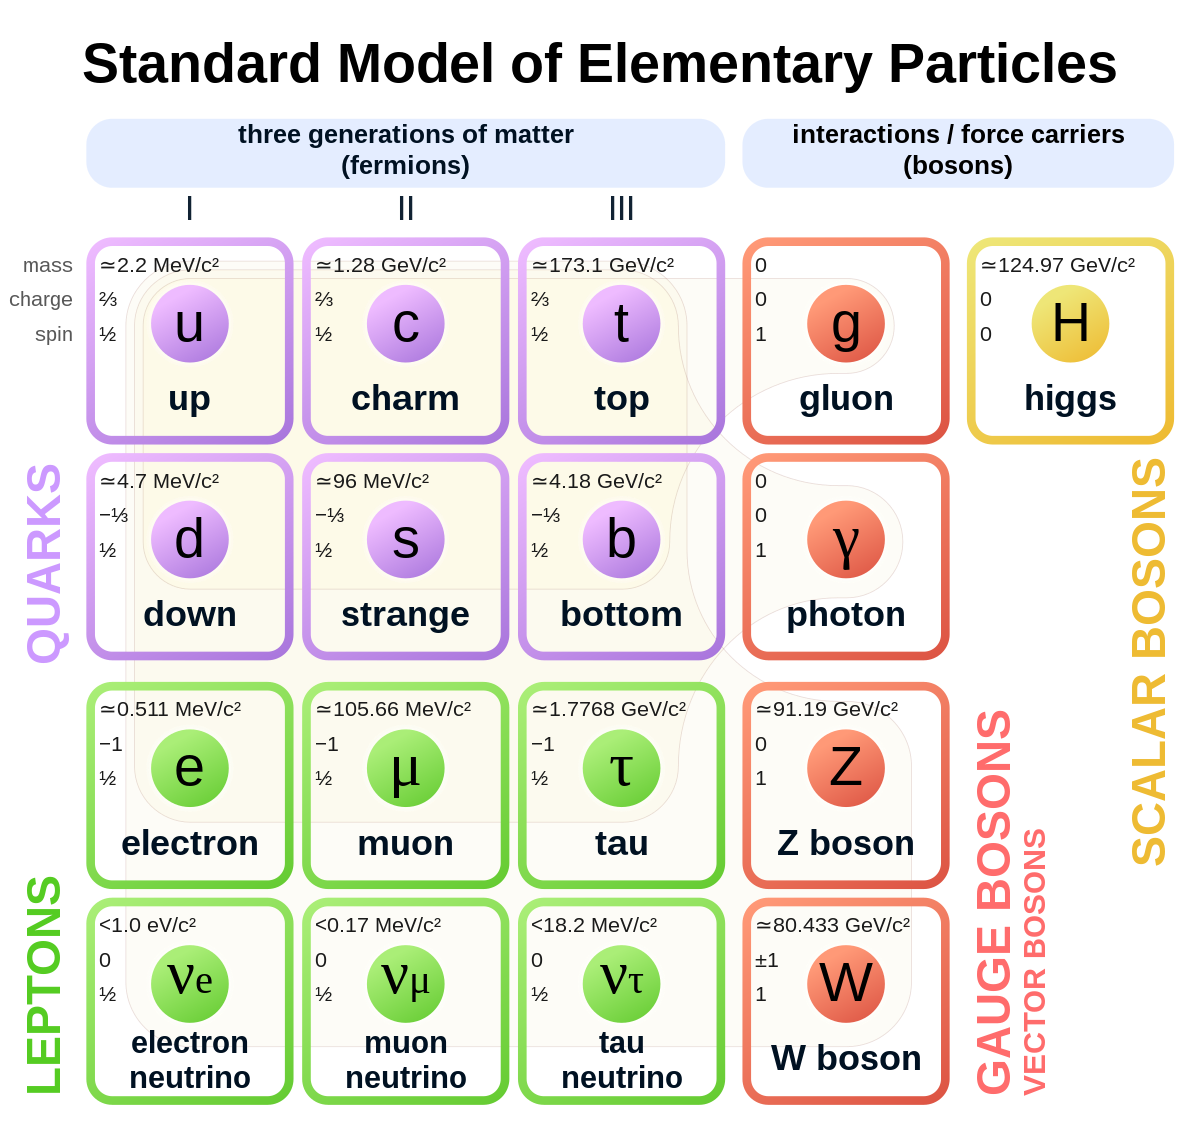
\includegraphics[width=0.6\linewidth]{Figures/StandardModel} 

}

\caption{Fig 1: A table representing all the particles in the Standard Model of physics. [Source](https://www.abc.net.au/news/science/2017-07-15/the-standard-model-of-particle-physics-explained/7670338)}\label{fig:Fig1}
\end{figure}

To prove the existence of the Higgs Boson, two detectors at CERN (ATLAS
and CMS) analyzed collisions between extremely high energy proton beams
generated by the LHC. Collisions between two high energy protons aren't
like collisions in the normal sense (such as a bat hitting a ball), but
they do share some similarities. In short, during a proton-proton
collision, the elementary particles marking up each (two up quarks and
one down quark, in this case) can interact with each other in order to
form other larger particles, which then decay into their own elementary
components. These kinds of interactions can be visualized by Feynman
Diagrams, and the rules used to draw them are dictated by conservation
laws within a field of physics known as Quantum Chromodynamics.

\begin{figure}

{\centering 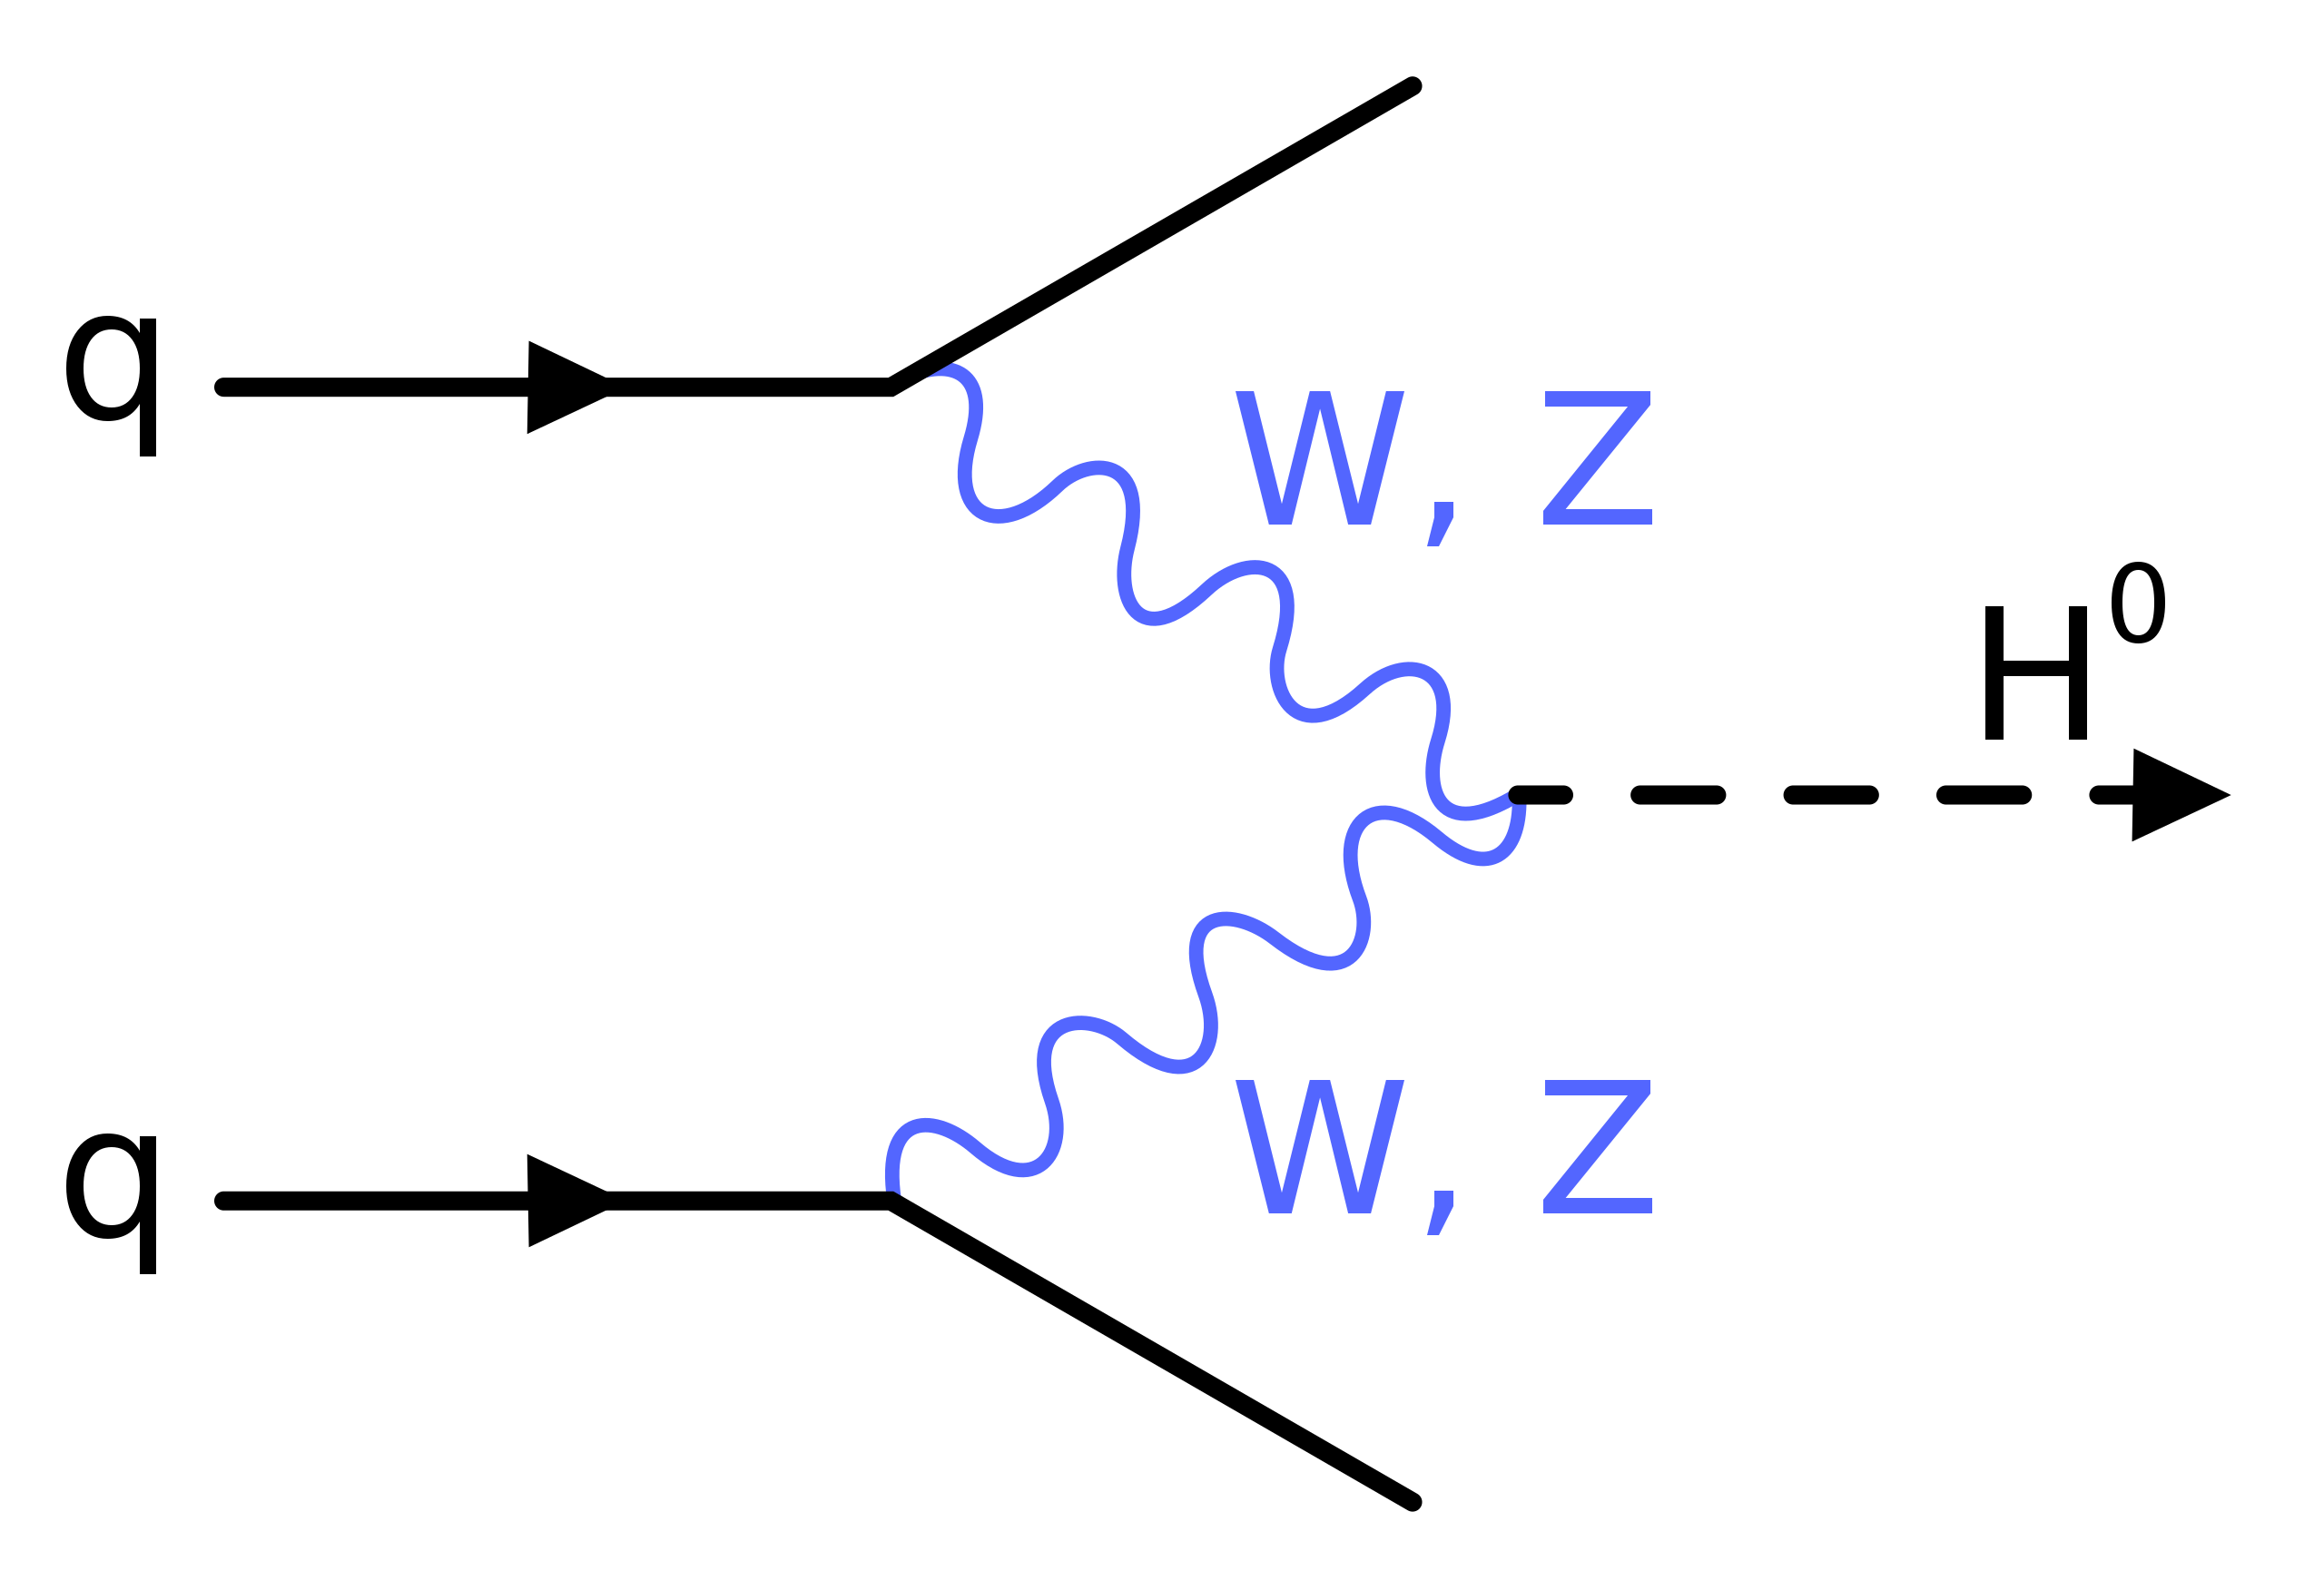
\includegraphics[width=0.6\linewidth]{Figures/Higgs_Feynman_Diagram} 

}

\caption{Fig 2: A feynman diagram showing a possible interaction during two quarks in a proton-proton collision. In this case the quakrs interact to form either W or Z bosons, which then further interact to emit a Higgs particle. [Source](https://www.wikiwand.com/en/Vector_boson)}\label{fig:Fig2}
\end{figure}

Inside the LHC, the streams of particles that are produced by these
interactions are called jets, considering that they all fly in roughly
the same direction.

\begin{figure}

{\centering 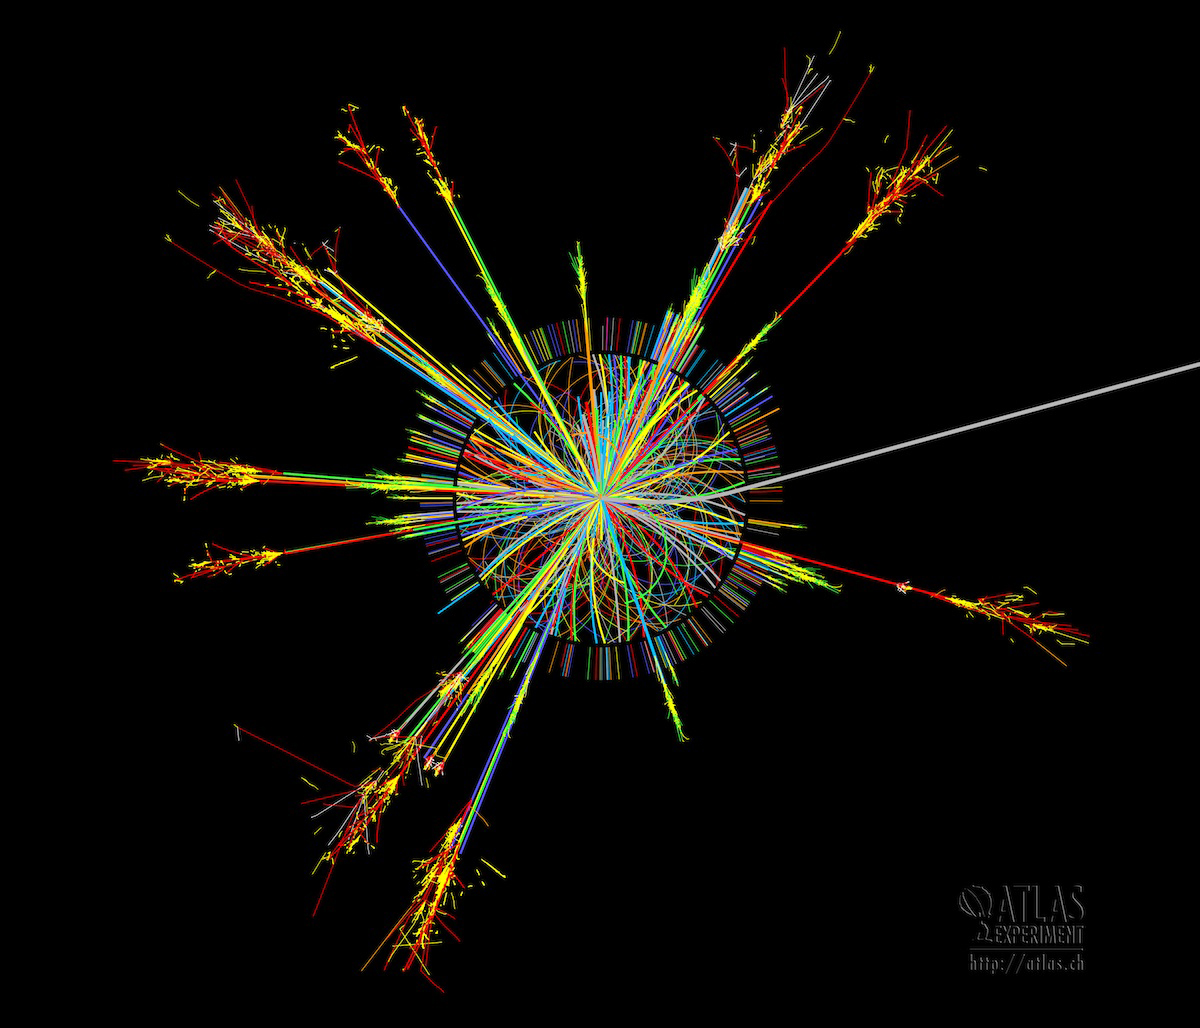
\includegraphics[width=0.6\linewidth]{Figures/Particle_Collision_Jets} 

}

\caption{Fig 3: A visualization of a proton-proton collision from the CERN ATLAS detector, in which ten particle jets are clearly visible. Each line represents a single particle. [Source](https://news.fnal.gov/2014/05/what-is-a-jet/)}\label{fig:Fig3}
\end{figure}

Analysis of one of these types of particle jets, known as \(b\)-jets,
was one of the ways that scientists at CERN were able to prove the
existence of the Higgs Boson. \(b\)-jets are those jets that originate
from a bottom quark, which is one of the elementary particles present in
a proton. While the Higgs boson's existence has already been proven,
scientists hypothesize that there are still a number of other unfounded
particles that could still be the result of interactions within a
\(b\)-jet. As such, identifying \(b\)-jets is of particular importance
to particle physics scientists.

\hypertarget{purpose}{%
\subsection{Purpose}\label{purpose}}

The goal of this project is to use data from proton-proton particle
collisions at CERN to determine whether or not there are certain
physical characteristics that are more likely to produce \(b\)-jets.
This will be done via a logistic regression methodology, which will be
used to predict whether or not a given collision produced a \(b\)-jet.
The data in this project comes from
\href{http://opendata.cern.ch/record/554}{CERN's open data portal} by
means of
\href{https://www.kaggle.com/datasets/fedesoriano/multijet-primary-dataset?q=CERN}{Kaggle},
and contains data from 21,726 proton-proton collisions. The data has
also been uploaded to
\href{https://raw.githubusercontent.com/williamzjasmine/CUNY_SPS_DS/master/DATA_606/Final_Project/MultiJetRun2010B.csv}{Github}.

\hypertarget{data-collection}{%
\section{Data Collection}\label{data-collection}}

The code chunk below imports the data from Github and stores it as an R
dataframe, \texttt{df}.

\begin{Shaded}
\begin{Highlighting}[]
\CommentTok{\# load data}
\NormalTok{link }\OtherTok{\textless{}{-}} \FunctionTok{getURL}\NormalTok{(}\StringTok{"https://raw.githubusercontent.com/williamzjasmine/CUNY\_SPS\_DS/master/DATA\_606/Final\_Project/MultiJetRun2010B.csv"}\NormalTok{)}
\NormalTok{df }\OtherTok{\textless{}{-}} \FunctionTok{read\_csv}\NormalTok{(link, }\AttributeTok{na=}\FunctionTok{c}\NormalTok{(}\StringTok{""}\NormalTok{, }\StringTok{"NA"}\NormalTok{))}
\FunctionTok{glimpse}\NormalTok{(df)}
\end{Highlighting}
\end{Shaded}

\begin{verbatim}
## Rows: 21,726
## Columns: 17
## $ Run    <dbl> 148029, 148029, 148029, 148029, 148029, 148029, 148029, 148029,~
## $ Lumi   <dbl> 388, 388, 388, 388, 388, 388, 388, 388, 388, 388, 388, 388, 388~
## $ Event  <dbl> 302318745, 302323641, 302336217, 302382289, 302403873, 30242079~
## $ MR     <dbl> 215.553, 155.437, 400.563, 286.245, 204.514, 263.468, 335.945, ~
## $ Rsq    <dbl> 0.03197660, 0.04215660, 0.02693840, 0.09419240, 0.01880400, 0.0~
## $ E1     <dbl> 136.7100, 83.3865, 253.1840, 175.4860, 833.7950, 604.4690, 685.~
## $ Px1    <dbl> -109.89300, 81.15000, 139.90200, -156.02400, 100.41000, -89.995~
## $ Py1    <dbl> -54.03420, 6.88361, 102.64000, -62.95350, -16.65900, 75.38630, ~
## $ Pz1    <dbl> -58.9032, -12.9688, -101.9350, -47.7434, -827.4980, 592.8480, -~
## $ E2     <dbl> 142.1790, 73.9025, 535.5510, 112.8510, 445.6120, 158.5160, 76.8~
## $ Px2    <dbl> 70.02540, -72.24720, -110.37900, 89.08430, -91.19910, 77.70750,~
## $ Py2    <dbl> 41.12250, 11.88350, -89.09290, 3.45025, 15.55830, -62.39290, -7~
## $ Pz2    <dbl> -116.51300, 3.08990, -516.17900, 67.90070, -390.14400, 122.2080~
## $ HT     <dbl> 203.666, 154.659, 343.280, 257.397, 269.492, 217.054, 175.667, ~
## $ MET    <dbl> 18.31100, 14.77470, 25.22110, 46.02880, 8.11345, 2.67841, 18.48~
## $ nJets  <dbl> 2, 2, 3, 2, 3, 2, 2, 2, 2, 3, 2, 3, 2, 2, 2, 4, 3, 2, 2, 2, 4, ~
## $ nBJets <dbl> 0, 0, 0, 0, 0, 0, 0, 0, 0, 0, 0, 0, 0, 0, 1, 0, 0, 1, 0, 0, 0, ~
\end{verbatim}

We see from the above output that the data was imported correctly and
that \texttt{df} includes all 21,726 proton-proton collisions. The below
chart includes a list of all the columns included, as well as a
description of each:

\begin{longtable}[]{@{}
  >{\raggedright\arraybackslash}p{(\columnwidth - 2\tabcolsep) * \real{0.5000}}
  >{\raggedright\arraybackslash}p{(\columnwidth - 2\tabcolsep) * \real{0.5000}}@{}}
\toprule()
\begin{minipage}[b]{\linewidth}\raggedright
Column Name
\end{minipage} & \begin{minipage}[b]{\linewidth}\raggedright
Description
\end{minipage} \\
\midrule()
\endhead
\texttt{Run} & The run number of the event. \\
\texttt{Lumi} & The lumi section of the event. \\
\texttt{Event} & The event number of the event. \\
\texttt{MR} & First razor kinematic variable, the MR variable is an
estimate of an overall mass scale, which in the limit of massless decay
products equals the mass of the heavy parent particle. \\
\texttt{Rsq} & Second razor kinematic variable, the Rsq variable is the
square of the ratio R, which quantifies the flow of energy in the plane
perpendicular to the beam and the partitioning of momentum between
visible and invisible particles. \\
\texttt{E1} & Energy of the leading megajet. \\
\texttt{Px1} & x-component of the momentum of the leading megajet. \\
\texttt{Py1} & y-component of the momentum of the leading megajet. \\
\texttt{Pz1} & z-component of the momentum of the leading megajet. \\
\texttt{E2} & Energy of the subleading megajet. \\
\texttt{Px2} & x-component of the momentum of the subleading megajet. \\
\texttt{Py2} & y-component of the momentum of the subleading megajet. \\
\texttt{Pz2} & z-component of the momentum of the subleading megajet. \\
\texttt{HT} & The scalar sum of the transverse momentum of the jets. \\
\texttt{MET} & The magnitude of the vector sum of the transverse energy
of the particles in the event. \\
\texttt{nJets} & The number of jets with transverse momentum above 40
GeV. \\
\texttt{nBJets} & The number of b-tagged jets with transverse momentum
above 40 GeV. \\
\bottomrule()
\end{longtable}

In this case, our response variable is \texttt{nBJets}, which counts the
number of \(b\)-jets present in each collision.

\hypertarget{data-cleaning}{%
\section{Data Cleaning}\label{data-cleaning}}

The first data cleaning step is to remove the \texttt{Run},
\texttt{Lumi}, and \texttt{Event} fields, which appear to be
documentation fields used at CERN, and add no predictive value.

\begin{Shaded}
\begin{Highlighting}[]
\NormalTok{df }\OtherTok{\textless{}{-}}\NormalTok{ df }\SpecialCharTok{\%\textgreater{}\%}
  \FunctionTok{select}\NormalTok{(}\SpecialCharTok{{-}}\NormalTok{Run, }\SpecialCharTok{{-}}\NormalTok{Lumi, }\SpecialCharTok{{-}}\NormalTok{Event)}
\end{Highlighting}
\end{Shaded}

Next, the code chunk below checks for any missing data:

\begin{Shaded}
\begin{Highlighting}[]
\FunctionTok{any}\NormalTok{(}\FunctionTok{is.na}\NormalTok{(df))}
\end{Highlighting}
\end{Shaded}

\begin{verbatim}
## [1] FALSE
\end{verbatim}

The remaining fields, with the exception of \texttt{nBJets}, represent
all the possible explanatory fields that we could use to predict our
response variable. However, we can use some physics knowledge to weed
out some of these fields.

The \texttt{E1}, \texttt{Px1}, \texttt{Py1}, \texttt{Pz1} and
\texttt{E2}, \texttt{Px2}, \texttt{Py2}, \texttt{Pz2} columns represent
the energy-momentum four vector \(p_{\mu}\) of the leading and
subleading megajets, respectively. These are the jets that have the
largest, and second largest total transverse momentum. This vector can
be written as

\[
\begin{equation}
p_u = (\frac{E}{c}, p_x, p_y, p_z)
\end{equation}
\]

where \(c\) is the speed of light and represents the special relatively
transformation of the more widely used space-time vector.

The below plot shows the relationship between each of the momentum
components (\(p_x\), \(p_y\), \(p_z\)) and the energy \(E\) of the
leading megajet by means of a scatterplot:

\begin{Shaded}
\begin{Highlighting}[]
\NormalTok{axes }\OtherTok{\textless{}{-}} \FunctionTok{c}\NormalTok{(}\StringTok{\textquotesingle{}x\textquotesingle{}}\NormalTok{, }\StringTok{\textquotesingle{}y\textquotesingle{}}\NormalTok{, }\StringTok{\textquotesingle{}z\textquotesingle{}}\NormalTok{)}
\NormalTok{component\_df }\OtherTok{\textless{}{-}} \FunctionTok{data.frame}\NormalTok{(}\FunctionTok{matrix}\NormalTok{(}\AttributeTok{ncol =} \DecValTok{3}\NormalTok{, }\AttributeTok{nrow =} \DecValTok{0}\NormalTok{))}
\FunctionTok{colnames}\NormalTok{(component\_df) }\OtherTok{\textless{}{-}} \FunctionTok{c}\NormalTok{(}\StringTok{\textquotesingle{}E1\textquotesingle{}}\NormalTok{, }\StringTok{\textquotesingle{}P1\textquotesingle{}}\NormalTok{, }\StringTok{\textquotesingle{}component\textquotesingle{}}\NormalTok{)}

\ControlFlowTok{for}\NormalTok{ (axis }\ControlFlowTok{in}\NormalTok{ axes) \{}
\NormalTok{  var\_name }\OtherTok{\textless{}{-}} \FunctionTok{paste}\NormalTok{(}\StringTok{"P"}\NormalTok{, axis, }\StringTok{"1"}\NormalTok{, }\AttributeTok{sep =} \StringTok{\textquotesingle{}\textquotesingle{}}\NormalTok{)}
\NormalTok{  tmp }\OtherTok{\textless{}{-}} \FunctionTok{cbind}\NormalTok{(df}\SpecialCharTok{$}\NormalTok{E1, df[var\_name])}
  \FunctionTok{colnames}\NormalTok{(tmp) }\OtherTok{\textless{}{-}} \FunctionTok{c}\NormalTok{(}\StringTok{\textquotesingle{}E1\textquotesingle{}}\NormalTok{, }\StringTok{\textquotesingle{}P1\textquotesingle{}}\NormalTok{)}
\NormalTok{  tmp }\OtherTok{\textless{}{-}}\NormalTok{ tmp }\SpecialCharTok{\%\textgreater{}\%} \FunctionTok{mutate}\NormalTok{(}\AttributeTok{component =}\NormalTok{ axis)}
\NormalTok{  component\_df }\OtherTok{\textless{}{-}} \FunctionTok{rbind}\NormalTok{(component\_df, tmp)}
\NormalTok{\}}

\FunctionTok{ggplot}\NormalTok{(}
  \AttributeTok{data =}\NormalTok{ component\_df, }
  \FunctionTok{aes}\NormalTok{(}\AttributeTok{x =}\NormalTok{ P1, }\AttributeTok{y =}\NormalTok{ E1, }\AttributeTok{fill =}\NormalTok{ component, }\AttributeTok{color =}\NormalTok{ component), }
\NormalTok{) }\SpecialCharTok{+}
  \FunctionTok{geom\_point}\NormalTok{(}
    \AttributeTok{alpha =} \FloatTok{0.35}\NormalTok{,}
    \AttributeTok{size =} \FloatTok{0.5}
\NormalTok{  ) }\SpecialCharTok{+} 
    \FunctionTok{labs}\NormalTok{(}
      \AttributeTok{x =} \StringTok{\textquotesingle{}Momentum (p)\textquotesingle{}}\NormalTok{,}
      \AttributeTok{y =} \StringTok{\textquotesingle{}Energy (E)\textquotesingle{}}\NormalTok{,}
\NormalTok{    )}
\end{Highlighting}
\end{Shaded}

\begin{figure}

{\centering \includegraphics[width=0.75\linewidth]{Final_Project_files/figure-latex/Ep_dot_plots-1} 

}

\caption{Fig 4: Scatterplot of energy and momentum component values for the leading megajet.}\label{fig:Ep_dot_plots}
\end{figure}

Given the structure of the points in the plot above, it is clear that
there appears to be a connection between these variables. It turns out
that we can use some simpler classical mechanics physics to define this
relationship. Given the kinetic energy (\(E = \frac{1}{2}mv^2\)) and
momentum (\(p = mv\)) of a particle, we can derive the following:

\[
\begin{align}
E &= \frac{1}{2}mv^2 \\
E &= \frac{m^2v^2}{2m} \\
E &= \frac{p^2}{2m}
\end{align}
\]

Since \(m\) (mass) is a constant, we see from the above that the energy
of the particle is proportional to the square of its momentum
(\(E \propto p^2\)). This proportionality that occurs in classical
physics is still present in relativity and quantum mechanics.

In our case, we can obtain a single scalar \(p\) value by using the
Pythagorean theorem on our vector components (note we cannot calculate
the true scalar value in this case since we lack the angles between the
components):

\[
\begin{align}
p^2 &\propto p_x^2+p_y^2+p_z^2 \\
p &\propto \sqrt{p_x^2+p_y^2+p_z^2} 
\end{align}
\]

The figure below calculates these scalar \(p\) values against the energy
values for both the leading and subleading megajet:

\begin{Shaded}
\begin{Highlighting}[]
\NormalTok{df }\OtherTok{\textless{}{-}}\NormalTok{ df }\SpecialCharTok{\%\textgreater{}\%} 
  \FunctionTok{mutate}\NormalTok{(}
    \AttributeTok{P1 =} \FunctionTok{sqrt}\NormalTok{((Px1 }\SpecialCharTok{*}\NormalTok{ Px1 }\SpecialCharTok{+}\NormalTok{ Py1 }\SpecialCharTok{*}\NormalTok{ Py1 }\SpecialCharTok{+}\NormalTok{ Pz1 }\SpecialCharTok{*}\NormalTok{ Pz1)),}
    \AttributeTok{P2 =} \FunctionTok{sqrt}\NormalTok{((Px2 }\SpecialCharTok{*}\NormalTok{ Px2 }\SpecialCharTok{+}\NormalTok{ Py2 }\SpecialCharTok{*}\NormalTok{ Py2 }\SpecialCharTok{+}\NormalTok{ Pz2 }\SpecialCharTok{*}\NormalTok{ Pz2))}
\NormalTok{  )}

\NormalTok{P\_df1 }\OtherTok{\textless{}{-}}\NormalTok{ df }\SpecialCharTok{\%\textgreater{}\%}
  \FunctionTok{select}\NormalTok{(E1, P1) }\SpecialCharTok{\%\textgreater{}\%}
    \FunctionTok{mutate}\NormalTok{(}\AttributeTok{jet\_type =} \StringTok{\textquotesingle{}Leading Megajet\textquotesingle{}}\NormalTok{)}
\FunctionTok{colnames}\NormalTok{(P\_df1) }\OtherTok{\textless{}{-}} \FunctionTok{c}\NormalTok{(}\StringTok{\textquotesingle{}E\textquotesingle{}}\NormalTok{, }\StringTok{\textquotesingle{}P\textquotesingle{}}\NormalTok{, }\StringTok{\textquotesingle{}jet\_type\textquotesingle{}}\NormalTok{)}
\NormalTok{P\_df2 }\OtherTok{\textless{}{-}}\NormalTok{ df }\SpecialCharTok{\%\textgreater{}\%}
  \FunctionTok{select}\NormalTok{(E2, P2) }\SpecialCharTok{\%\textgreater{}\%}
    \FunctionTok{mutate}\NormalTok{(}\AttributeTok{jet\_type =} \StringTok{\textquotesingle{}Subleading Megajet\textquotesingle{}}\NormalTok{)}
\FunctionTok{colnames}\NormalTok{(P\_df2) }\OtherTok{\textless{}{-}} \FunctionTok{c}\NormalTok{(}\StringTok{\textquotesingle{}E\textquotesingle{}}\NormalTok{, }\StringTok{\textquotesingle{}P\textquotesingle{}}\NormalTok{, }\StringTok{\textquotesingle{}jet\_type\textquotesingle{}}\NormalTok{)}
\NormalTok{P\_df }\OtherTok{\textless{}{-}} \FunctionTok{rbind}\NormalTok{(P\_df1, P\_df2)}


\FunctionTok{ggplot}\NormalTok{(}
  \AttributeTok{data =}\NormalTok{ P\_df, }
  \FunctionTok{aes}\NormalTok{(}\AttributeTok{x =} \FunctionTok{sqrt}\NormalTok{(P), }\AttributeTok{y =}\NormalTok{ E, }\AttributeTok{fill =}\NormalTok{ jet\_type, }\AttributeTok{color =}\NormalTok{ jet\_type), }
\NormalTok{) }\SpecialCharTok{+}
  \FunctionTok{geom\_point}\NormalTok{(}
    \AttributeTok{alpha =} \FloatTok{0.5}\NormalTok{,}
    \AttributeTok{size =} \DecValTok{1}\NormalTok{,}
\NormalTok{  ) }\SpecialCharTok{+} 
  \FunctionTok{stat\_smooth}\NormalTok{(}
    \AttributeTok{method =} \StringTok{"lm"}\NormalTok{,}
    \AttributeTok{formula =}\NormalTok{ y }\SpecialCharTok{\textasciitilde{}} \FunctionTok{poly}\NormalTok{(x, }\DecValTok{2}\NormalTok{),}
    \AttributeTok{se =} \ConstantTok{FALSE}\NormalTok{,}
    \AttributeTok{color =} \StringTok{\textquotesingle{}black\textquotesingle{}}\NormalTok{,}
    \AttributeTok{size =} \FloatTok{0.25}
\NormalTok{  ) }\SpecialCharTok{+}
    \FunctionTok{labs}\NormalTok{(}
      \AttributeTok{x =} \StringTok{\textquotesingle{}Momentum (p)\textquotesingle{}}\NormalTok{,}
      \AttributeTok{y =} \StringTok{\textquotesingle{}Energy (E)\textquotesingle{}}\NormalTok{,}
\NormalTok{    )}
\end{Highlighting}
\end{Shaded}

\begin{figure}

{\centering \includegraphics[width=0.75\linewidth]{Final_Project_files/figure-latex/Ep-fit-1} 

}

\caption{Fig 5: Relationship between energy and scalar momentum for both leading and subleading megajets. The black line repesents a polynomial fit of degree 2.}\label{fig:Ep-fit}
\end{figure}

Based on the figure above, we can see the how well a quadratic fit
aligns to the data, clearly exhibiting the \(E \propto p^2\)
proportionality mentioned earlier.

Because these variables have a clear connection with one another, we
cannot view them as independent and must remove all but one in order to
have cleaner model. This is done in the cell below, which removes all
the momentum component variables (leaving only \(E1\) and \(E2\) as the
remaining energy-momentum vector variables):

\begin{Shaded}
\begin{Highlighting}[]
\NormalTok{df }\OtherTok{\textless{}{-}}\NormalTok{ df }\SpecialCharTok{\%\textgreater{}\%}
  \FunctionTok{select}\NormalTok{(}\SpecialCharTok{{-}}\FunctionTok{contains}\NormalTok{(}\StringTok{\textquotesingle{}P\textquotesingle{}}\NormalTok{))}
\end{Highlighting}
\end{Shaded}

To perform the next data cleaning step, the cell below creates dot plots
of all pairs of remaining independent variables:

\begin{Shaded}
\begin{Highlighting}[]
\NormalTok{df }\SpecialCharTok{\%\textgreater{}\%}
  \FunctionTok{select}\NormalTok{(}\SpecialCharTok{{-}}\FunctionTok{contains}\NormalTok{(}\StringTok{\textquotesingle{}P\textquotesingle{}}\NormalTok{), }\SpecialCharTok{{-}}\FunctionTok{contains}\NormalTok{(}\StringTok{\textquotesingle{}Jet\textquotesingle{}}\NormalTok{)) }\SpecialCharTok{\%\textgreater{}\%}
    \FunctionTok{ggpairs}\NormalTok{(}\AttributeTok{axisLabels =} \StringTok{\textquotesingle{}none\textquotesingle{}}\NormalTok{)}
\end{Highlighting}
\end{Shaded}

\begin{figure}

{\centering \includegraphics[width=1\linewidth]{Final_Project_files/figure-latex/plotpairsv1-1} 

}

\caption{Fig 6: Scatter plots for all remaining independent variables.}\label{fig:plotpairsv1}
\end{figure}

We can see that there are a number of variables that do exhibit some
high correlation values, which are visually evidenced in the
scatterplots. The two variables that appear to be driving the highest
correlation values (\texttt{Rsq} and \texttt{MR}) are removed in the
cell below:

\begin{Shaded}
\begin{Highlighting}[]
\NormalTok{df }\OtherTok{\textless{}{-}}\NormalTok{ df }\SpecialCharTok{\%\textgreater{}\%}
  \FunctionTok{select}\NormalTok{(}\SpecialCharTok{{-}}\NormalTok{MR, }\SpecialCharTok{{-}}\NormalTok{Rsq)}
\end{Highlighting}
\end{Shaded}

We can now recreate the all the remaining scatterplots:

\begin{Shaded}
\begin{Highlighting}[]
\NormalTok{df }\SpecialCharTok{\%\textgreater{}\%}
  \FunctionTok{select}\NormalTok{(}\SpecialCharTok{{-}}\FunctionTok{contains}\NormalTok{(}\StringTok{\textquotesingle{}P\textquotesingle{}}\NormalTok{), }\SpecialCharTok{{-}}\FunctionTok{contains}\NormalTok{(}\StringTok{\textquotesingle{}Jet\textquotesingle{}}\NormalTok{)) }\SpecialCharTok{\%\textgreater{}\%}
    \FunctionTok{ggpairs}\NormalTok{(}\AttributeTok{axisLabels =} \StringTok{\textquotesingle{}none\textquotesingle{}}\NormalTok{)}
\end{Highlighting}
\end{Shaded}

\begin{figure}

{\centering \includegraphics[width=1\linewidth]{Final_Project_files/figure-latex/plotpairsv2-1} 

}

\caption{Fig 7: Scatter plots for all remaining independent variables with MR and Rsq variables removed.}\label{fig:plotpairsv2}
\end{figure}

These correlation values seem to be within a reasonable means to include
in our forthcoming analysis and modelling.

\hypertarget{data-analysis}{%
\section{Data Analysis}\label{data-analysis}}

Now that we have settled on a final set of independent variables, we can
perform some exploratory data analysis to get a better look at our data.

The code chunk below provides summary statistics for all the fields in
\texttt{df}:

\begin{Shaded}
\begin{Highlighting}[]
\FunctionTok{summary}\NormalTok{(df)}
\end{Highlighting}
\end{Shaded}

\begin{verbatim}
##        E1                E2                HT              MET          
##  Min.   :  44.95   Min.   :  42.05   Min.   : 120.9   Min.   :  0.1004  
##  1st Qu.: 143.53   1st Qu.: 126.92   1st Qu.: 193.3   1st Qu.:  8.6268  
##  Median : 212.06   Median : 204.14   Median : 223.7   Median : 14.0350  
##  Mean   : 297.18   Mean   : 277.41   Mean   : 242.3   Mean   : 16.0054  
##  3rd Qu.: 374.54   3rd Qu.: 366.71   3rd Qu.: 269.2   3rd Qu.: 21.0910  
##  Max.   :2101.58   Max.   :1843.36   Max.   :1462.6   Max.   :423.1440  
##      nJets           nBJets       
##  Min.   :2.000   Min.   :0.00000  
##  1st Qu.:2.000   1st Qu.:0.00000  
##  Median :2.000   Median :0.00000  
##  Mean   :2.436   Mean   :0.05367  
##  3rd Qu.:3.000   3rd Qu.:0.00000  
##  Max.   :7.000   Max.   :2.00000
\end{verbatim}

Next, the cell below shows the distribution of the number of \(b\)-jets
in each collision.

\begin{Shaded}
\begin{Highlighting}[]
\FunctionTok{ggplot}\NormalTok{(}\AttributeTok{data =}\NormalTok{ df, }\FunctionTok{aes}\NormalTok{(}\AttributeTok{x =}\NormalTok{ nBJets)) }\SpecialCharTok{+}
  \FunctionTok{geom\_histogram}\NormalTok{(}\AttributeTok{bins =} \FunctionTok{length}\NormalTok{(}\FunctionTok{unique}\NormalTok{(df}\SpecialCharTok{$}\NormalTok{nBJets))) }\SpecialCharTok{+} 
    \FunctionTok{labs}\NormalTok{(}
      \AttributeTok{x =} \StringTok{\textquotesingle{}Number of b{-}Jets\textquotesingle{}}\NormalTok{,}
      \AttributeTok{y =} \StringTok{\textquotesingle{}Count\textquotesingle{}}\NormalTok{,}
\NormalTok{    )}
\end{Highlighting}
\end{Shaded}

\begin{figure}

{\centering \includegraphics[width=0.75\linewidth]{Final_Project_files/figure-latex/bjets_dist-1} 

}

\caption{Fig 8: Distribution of the number of b-jets in each collision.}\label{fig:bjets_dist}
\end{figure}

As is clear from the data above, \(b\)-jets are pretty rare in the
particle collisions included in our dataset. Most collisions have none,
and the most \(b\)-jets observed in a single collision is two. Given
this distribution, it makes sense to transform our response variable
into a binary variable \texttt{BJet} such that \texttt{BJet\ =\ 1} if a
collision produced and \(b\)-jet, and \texttt{Bjet} = 0 if not. This is
done in the cell below:

\begin{Shaded}
\begin{Highlighting}[]
\NormalTok{df }\OtherTok{\textless{}{-}}\NormalTok{ df }\SpecialCharTok{\%\textgreater{}\%} 
  \FunctionTok{mutate}\NormalTok{(}\AttributeTok{BJet =} \FunctionTok{ifelse}\NormalTok{(nBJets }\SpecialCharTok{\textgreater{}=} \DecValTok{1}\NormalTok{, }\DecValTok{1}\NormalTok{, }\DecValTok{0}\NormalTok{))}
\end{Highlighting}
\end{Shaded}

Next, the cell below shows the distribution of \texttt{nJets}, to see
how it compares to the distribution in Fig 8.

\begin{Shaded}
\begin{Highlighting}[]
\FunctionTok{ggplot}\NormalTok{(}\AttributeTok{data =}\NormalTok{ df, }\FunctionTok{aes}\NormalTok{(}\AttributeTok{x =}\NormalTok{ nJets)) }\SpecialCharTok{+}
  \FunctionTok{geom\_histogram}\NormalTok{(}\AttributeTok{bins =} \FunctionTok{length}\NormalTok{(}\FunctionTok{unique}\NormalTok{(df}\SpecialCharTok{$}\NormalTok{nJets))) }\SpecialCharTok{+} 
    \FunctionTok{labs}\NormalTok{(}
      \AttributeTok{x =} \StringTok{\textquotesingle{}Number of Jets in collision\textquotesingle{}}\NormalTok{,}
      \AttributeTok{y =} \StringTok{\textquotesingle{}Count of Collisions\textquotesingle{}}
\NormalTok{    )}
\end{Highlighting}
\end{Shaded}

\begin{figure}

{\centering \includegraphics[width=0.75\linewidth]{Final_Project_files/figure-latex/njets_dist-1} 

}

\caption{Fig 9: Distribution of the number of jets in each collision.}\label{fig:njets_dist}
\end{figure}

As we can see from the distribution, each collision has at least two
jets (which makes sense, given a collision requires there be at least
one interaction), but that there are never more than 6.

The cell below determines exactly just how rare these \(b\)-jets are:

\begin{Shaded}
\begin{Highlighting}[]
\NormalTok{pBJet }\OtherTok{\textless{}{-}} \FunctionTok{round}\NormalTok{((}\FunctionTok{sum}\NormalTok{(df}\SpecialCharTok{$}\NormalTok{nBJets) }\SpecialCharTok{/} \FunctionTok{sum}\NormalTok{(df}\SpecialCharTok{$}\NormalTok{nJets)) }\SpecialCharTok{*} \DecValTok{100}\NormalTok{, }\AttributeTok{digits =} \DecValTok{2}\NormalTok{)}
\NormalTok{pBJet\_c }\OtherTok{\textless{}{-}} \FunctionTok{round}\NormalTok{((}\FunctionTok{sum}\NormalTok{(df}\SpecialCharTok{$}\NormalTok{BJet) }\SpecialCharTok{/} \FunctionTok{nrow}\NormalTok{(df)) }\SpecialCharTok{*} \DecValTok{100}\NormalTok{, }\AttributeTok{digits =} \DecValTok{2}\NormalTok{)}
\NormalTok{nBJet }\OtherTok{\textless{}{-}} \FunctionTok{unname}\NormalTok{(}\FunctionTok{table}\NormalTok{(df}\SpecialCharTok{$}\NormalTok{BJet))[}\DecValTok{2}\NormalTok{]}
\end{Highlighting}
\end{Shaded}

\textbf{Percentage of observed particle jets that were \(b\)-jets =}
2.2\% \textbf{Percentage of collisions that observed a \(b\)-jet =}
5.11\% \textbf{Number of collisions that observed a \(b\)-jet = } 1111

\hypertarget{modelling}{%
\section{Modelling}\label{modelling}}

\hypertarget{create-initial-model}{%
\subsection{Create Initial Model}\label{create-initial-model}}

Given the binary nature of the response variable, we will use logistic
regression to attempt to predict if a collision results in a \(b\)-jet.
The code chunk below creates a logistic model using data from all the
collisions in \texttt{df}:

\begin{Shaded}
\begin{Highlighting}[]
\NormalTok{model }\OtherTok{\textless{}{-}} \FunctionTok{glm}\NormalTok{(BJet }\SpecialCharTok{\textasciitilde{}}\NormalTok{ E1 }\SpecialCharTok{+}\NormalTok{ E2 }\SpecialCharTok{+}\NormalTok{ HT }\SpecialCharTok{+}\NormalTok{ MET, }\AttributeTok{family=}\FunctionTok{binomial}\NormalTok{(}\AttributeTok{link=}\StringTok{\textquotesingle{}logit\textquotesingle{}}\NormalTok{), }\AttributeTok{data=}\NormalTok{df)}
\FunctionTok{summary}\NormalTok{(model)}
\end{Highlighting}
\end{Shaded}

\begin{verbatim}
## 
## Call:
## glm(formula = BJet ~ E1 + E2 + HT + MET, family = binomial(link = "logit"), 
##     data = df)
## 
## Deviance Residuals: 
##     Min       1Q   Median       3Q      Max  
## -1.9805  -0.3443  -0.3172  -0.2820   2.8828  
## 
## Coefficients:
##               Estimate Std. Error z value Pr(>|z|)    
## (Intercept) -3.3728408  0.0923828 -36.509  < 2e-16 ***
## E1          -0.0006706  0.0001579  -4.247 2.17e-05 ***
## E2          -0.0010198  0.0001791  -5.693 1.25e-08 ***
## HT           0.0029724  0.0003627   8.195 2.51e-16 ***
## MET          0.0105801  0.0024607   4.300 1.71e-05 ***
## ---
## Signif. codes:  0 '***' 0.001 '**' 0.01 '*' 0.05 '.' 0.1 ' ' 1
## 
## (Dispersion parameter for binomial family taken to be 1)
## 
##     Null deviance: 8770.8  on 21725  degrees of freedom
## Residual deviance: 8657.1  on 21721  degrees of freedom
## AIC: 8667.1
## 
## Number of Fisher Scoring iterations: 6
\end{verbatim}

Before we go about analyzing performance and making predictions, we will
use this initial model to perform diagnostics and check all of our
assumptions for logistic regression.

\hypertarget{assumptions}{%
\subsection{Assumptions}\label{assumptions}}

\hypertarget{independent-observations}{%
\subsubsection{Independent
Observations}\label{independent-observations}}

Each of the rows in our dataset represent data from individual
collisions and the results of one collision have no effect on the
results of another. As such, we can conclude each collision is
independent and this assumption is satisfied.

\hypertarget{no-multicollinearity-among-explanatory-variables}{%
\subsubsection{No Multicollinearity Among Explanatory
Variables}\label{no-multicollinearity-among-explanatory-variables}}

While this was in a sense already checked in our data analysis section
by observing Fig 7, we can use our initial model to calculate the
variance inflation factor (VIF) values for each explanatory variable to
further confirm this condition is satisfied. for multicollinearity:

\begin{Shaded}
\begin{Highlighting}[]
\FunctionTok{vif}\NormalTok{(model)}
\end{Highlighting}
\end{Shaded}

\begin{verbatim}
##       E1       E2       HT      MET 
## 1.127792 1.147190 1.349789 1.062291
\end{verbatim}

VIF numbers provide a quantitative measure of how much one explanatory
variable is correlated to any others,
\href{https://www.ncbi.nlm.nih.gov/pmc/articles/PMC5993839/}{and
typically any value below 2.5 is low enough for the lack of
multicollinearity assumption to be met}. The output above shows that
this is the case for all of our independent variables.

\hypertarget{no-extreme-outliers}{%
\subsubsection{No Extreme Outliers}\label{no-extreme-outliers}}

The next condition for logistic regression is that the independent
variables contain no extreme outliers. We first check this using the
simple definition that an outlier is any value that is 1.5 times the IQR
over the third quartile or 1.5 times the IQR below the first quartile.
This is done in the cell below for each of our independent variables.

\begin{Shaded}
\begin{Highlighting}[]
\NormalTok{col\_check }\OtherTok{=} \FunctionTok{c}\NormalTok{()}
\NormalTok{loop\_data }\OtherTok{=} \FunctionTok{select}\NormalTok{(df, E1, E2, HT, MET)}

\ControlFlowTok{for}\NormalTok{(i }\ControlFlowTok{in} \DecValTok{1}\SpecialCharTok{:}\FunctionTok{ncol}\NormalTok{(loop\_data)) \{       }
\NormalTok{  col\_data }\OtherTok{\textless{}{-}} \FunctionTok{as.matrix}\NormalTok{(loop\_data[ , i])}
\NormalTok{  iqr }\OtherTok{\textless{}{-}} \FunctionTok{IQR}\NormalTok{(col\_data)}
\NormalTok{  q1 }\OtherTok{\textless{}{-}} \FunctionTok{unname}\NormalTok{(}\FunctionTok{quantile}\NormalTok{(col\_data))[}\DecValTok{2}\NormalTok{]}
\NormalTok{  q3 }\OtherTok{\textless{}{-}} \FunctionTok{unname}\NormalTok{(}\FunctionTok{quantile}\NormalTok{(col\_data))[}\DecValTok{4}\NormalTok{]}
\NormalTok{  outliers }\OtherTok{\textless{}{-}} 
    \FunctionTok{any}\NormalTok{(}
\NormalTok{      col\_data }\SpecialCharTok{\textgreater{}}\NormalTok{ (}\FloatTok{1.5} \SpecialCharTok{*}\NormalTok{ iqr) }\SpecialCharTok{+}\NormalTok{ q3 }\SpecialCharTok{|}
\NormalTok{      col\_data }\SpecialCharTok{\textless{}}\NormalTok{ q1 }\SpecialCharTok{{-}}\NormalTok{ (}\FloatTok{1.5} \SpecialCharTok{*}\NormalTok{ iqr)}
\NormalTok{    )}
\NormalTok{  col\_check }\OtherTok{\textless{}{-}} \FunctionTok{append}\NormalTok{(col\_check, outliers)}
\NormalTok{\}}

\NormalTok{col\_check}
\end{Highlighting}
\end{Shaded}

\begin{verbatim}
## [1] TRUE TRUE TRUE TRUE
\end{verbatim}

By this definition, each of our four columns have outliers. As such, we
can use our model to remove these points by calculating Cook's Distance.
Cook's distance is a metric that is used to determine how much influence
a single data point holds over a model's performance
\href{https://www.jstor.org/stable/1268249}{by measuring how that
model's predicted values would change if it didn't exist}. As such, it
can be used to identify and remove problematic outliers. Typically, the
threshold used for removal is if Cook's distance is greater than
\(\frac{4}{n}\), where \(n\) is the number of observations in our
dataset. The plot below shows the cook's distance for all of the
observations in our training set:

\begin{Shaded}
\begin{Highlighting}[]
\NormalTok{cooksD }\OtherTok{\textless{}{-}} \FunctionTok{cooks.distance}\NormalTok{(model)}
\NormalTok{cooks }\OtherTok{\textless{}{-}} \FunctionTok{as.data.frame}\NormalTok{(cooksD)}
\FunctionTok{colnames}\NormalTok{(cooks) }\OtherTok{\textless{}{-}} \FunctionTok{c}\NormalTok{(}\StringTok{\textquotesingle{}d\_c\textquotesingle{}}\NormalTok{)}
\NormalTok{cooks}\SpecialCharTok{$}\NormalTok{row\_num }\OtherTok{\textless{}{-}} \FunctionTok{seq.int}\NormalTok{(}\FunctionTok{nrow}\NormalTok{(cooks)) }

\FunctionTok{ggplot}\NormalTok{(}\AttributeTok{data =}\NormalTok{ cooks, }\FunctionTok{aes}\NormalTok{(}\AttributeTok{x =}\NormalTok{ row\_num, }\AttributeTok{y =}\NormalTok{ d\_c)) }\SpecialCharTok{+} 
  \FunctionTok{geom\_point}\NormalTok{(}\AttributeTok{size =}  \DecValTok{1}\NormalTok{) }\SpecialCharTok{+}
    \FunctionTok{geom\_hline}\NormalTok{(}\AttributeTok{yintercept =} \DecValTok{4} \SpecialCharTok{/} \FunctionTok{nrow}\NormalTok{(df), }\AttributeTok{color =} \StringTok{"red"}\NormalTok{) }\SpecialCharTok{+}
      \FunctionTok{labs}\NormalTok{(}
        \AttributeTok{x =} \StringTok{"Index"}\NormalTok{,}
        \AttributeTok{y =} \StringTok{"Cook\textquotesingle{}s Distance"}
\NormalTok{      ) }\SpecialCharTok{+} 
        \FunctionTok{ylim}\NormalTok{(}\DecValTok{0}\NormalTok{, }\FloatTok{0.002}\NormalTok{)}
\end{Highlighting}
\end{Shaded}

\begin{figure}

{\centering \includegraphics[width=0.75\linewidth]{Final_Project_files/figure-latex/check-outliers-cook-1} 

}

\caption{Fig 10: Cook distance plotted for all observations. The line represents the 4 / n threshold, over which any observation is considered an outlier.}\label{fig:check-outliers-cook}
\end{figure}

As is clear from the plot above, the data seems grouped into a two
distinct sets, with one of those containing a large number of outliers.
To do further analyses on these points, we can separate our data into
two new dataframes \texttt{outlier\_df}, \texttt{no\_outlier\_df}:

\begin{Shaded}
\begin{Highlighting}[]
\NormalTok{influential\_obs }\OtherTok{\textless{}{-}} \FunctionTok{as.numeric}\NormalTok{(}\FunctionTok{names}\NormalTok{(cooksD)[(cooksD }\SpecialCharTok{\textgreater{}}\NormalTok{ (}\DecValTok{4}\SpecialCharTok{/}\FunctionTok{nrow}\NormalTok{(df)))])}
\NormalTok{no\_outliers\_df }\OtherTok{\textless{}{-}}\NormalTok{ df[}\SpecialCharTok{{-}}\NormalTok{influential\_obs, ]}
\NormalTok{outliers\_df }\OtherTok{\textless{}{-}}\NormalTok{ df[influential\_obs, ]}

\FunctionTok{nrow}\NormalTok{(outliers\_df)}
\end{Highlighting}
\end{Shaded}

\begin{verbatim}
## [1] 1140
\end{verbatim}

The output above shows that using the Cook's distance methodology, 1,140
outliers have been identified. However, when we look at the counts of
the response variable in each of these newly created dataframes:

\begin{Shaded}
\begin{Highlighting}[]
\FunctionTok{table}\NormalTok{(no\_outliers\_df}\SpecialCharTok{$}\NormalTok{BJet)}
\end{Highlighting}
\end{Shaded}

\begin{verbatim}
## 
##     0     1 
## 20585     1
\end{verbatim}

\begin{Shaded}
\begin{Highlighting}[]
\FunctionTok{table}\NormalTok{(outliers\_df}\SpecialCharTok{$}\NormalTok{BJet)}
\end{Highlighting}
\end{Shaded}

\begin{verbatim}
## 
##    0    1 
##   30 1110
\end{verbatim}

we see that the outliers dataframe includes almost every single
collision in which there was a \(b\)-jet. As such, we should not remove
these outliers when creating our model so that it can still have
predictive power.

\hypertarget{linear-relationship-between-explanatory-variables-and-the-logit-of-the-response-variable}{%
\subsubsection{Linear Relationship Between Explanatory Variables and the
Logit of the Response
Variable}\label{linear-relationship-between-explanatory-variables-and-the-logit-of-the-response-variable}}

To ensure this condition is met, the cell below calculates the log odds
of each of the probabilities determined by the model. Given a
probability \(p\), the log odds or logit of \(p\) are:

\[
\begin{equation}
\text{logit}(p) = \log \left( \frac{p}{1-p} \right)
\end{equation}
\]

These logit values are plotted below in scatter plots with each of our
independent variables:

\begin{Shaded}
\begin{Highlighting}[]
\NormalTok{probs }\OtherTok{\textless{}{-}} \FunctionTok{predict}\NormalTok{(model, }\AttributeTok{type =} \StringTok{\textquotesingle{}response\textquotesingle{}}\NormalTok{)}

\NormalTok{logit }\OtherTok{\textless{}{-}} \FunctionTok{log}\NormalTok{(probs}\SpecialCharTok{/}\NormalTok{(}\DecValTok{1}\SpecialCharTok{{-}}\NormalTok{probs))}

\NormalTok{E1\_plot }\OtherTok{\textless{}{-}}
  \FunctionTok{ggplot}\NormalTok{(}\AttributeTok{data =}\NormalTok{ df, }\FunctionTok{aes}\NormalTok{(}\AttributeTok{x =}\NormalTok{ logit, }\AttributeTok{y =}\NormalTok{ E1)) }\SpecialCharTok{+} 
    \FunctionTok{geom\_point}\NormalTok{() }\SpecialCharTok{+}
      \FunctionTok{geom\_smooth}\NormalTok{(}\AttributeTok{method =} \StringTok{\textquotesingle{}lm\textquotesingle{}}\NormalTok{) }\SpecialCharTok{+} 
        \FunctionTok{labs}\NormalTok{(}
          \AttributeTok{x =} \StringTok{\textquotesingle{}Logit\textquotesingle{}}\NormalTok{,}
          \AttributeTok{y =} \StringTok{\textquotesingle{}E1\textquotesingle{}}
\NormalTok{        ) }\SpecialCharTok{+} 
          \FunctionTok{theme}\NormalTok{(}
            \AttributeTok{axis.text.x=}\FunctionTok{element\_blank}\NormalTok{(),}
            \AttributeTok{axis.text.y=}\FunctionTok{element\_blank}\NormalTok{()}
\NormalTok{          )}
\NormalTok{E2\_plot }\OtherTok{\textless{}{-}}
  \FunctionTok{ggplot}\NormalTok{(}\AttributeTok{data =}\NormalTok{ df, }\FunctionTok{aes}\NormalTok{(}\AttributeTok{x =}\NormalTok{ logit, }\AttributeTok{y =}\NormalTok{ E2)) }\SpecialCharTok{+} 
    \FunctionTok{geom\_point}\NormalTok{() }\SpecialCharTok{+}
      \FunctionTok{geom\_smooth}\NormalTok{(}\AttributeTok{method =} \StringTok{\textquotesingle{}lm\textquotesingle{}}\NormalTok{) }\SpecialCharTok{+}         
        \FunctionTok{labs}\NormalTok{(}
          \AttributeTok{x =} \StringTok{\textquotesingle{}Logit\textquotesingle{}}\NormalTok{,}
          \AttributeTok{y =} \StringTok{\textquotesingle{}E2\textquotesingle{}}
\NormalTok{        ) }\SpecialCharTok{+} 
          \FunctionTok{theme}\NormalTok{(}
            \AttributeTok{axis.text.x=}\FunctionTok{element\_blank}\NormalTok{(),}
            \AttributeTok{axis.text.y=}\FunctionTok{element\_blank}\NormalTok{()}
\NormalTok{          )}
\NormalTok{HT\_plot }\OtherTok{\textless{}{-}}
  \FunctionTok{ggplot}\NormalTok{(}\AttributeTok{data =}\NormalTok{ df, }\FunctionTok{aes}\NormalTok{(}\AttributeTok{x =}\NormalTok{ logit, }\AttributeTok{y =}\NormalTok{ HT)) }\SpecialCharTok{+} 
    \FunctionTok{geom\_point}\NormalTok{() }\SpecialCharTok{+}
      \FunctionTok{geom\_smooth}\NormalTok{(}\AttributeTok{method =} \StringTok{\textquotesingle{}lm\textquotesingle{}}\NormalTok{) }\SpecialCharTok{+} 
        \FunctionTok{labs}\NormalTok{(}
          \AttributeTok{x =} \StringTok{\textquotesingle{}Logit\textquotesingle{}}\NormalTok{,}
          \AttributeTok{y =} \StringTok{\textquotesingle{}HT\textquotesingle{}}
\NormalTok{        ) }\SpecialCharTok{+} 
          \FunctionTok{theme}\NormalTok{(}
            \AttributeTok{axis.text.x=}\FunctionTok{element\_blank}\NormalTok{(),}
            \AttributeTok{axis.text.y=}\FunctionTok{element\_blank}\NormalTok{()}
\NormalTok{          )}
\NormalTok{MET\_plot }\OtherTok{\textless{}{-}}
  \FunctionTok{ggplot}\NormalTok{(}\AttributeTok{data =}\NormalTok{ df, }\FunctionTok{aes}\NormalTok{(}\AttributeTok{x =}\NormalTok{ logit, }\AttributeTok{y =}\NormalTok{ MET)) }\SpecialCharTok{+} 
    \FunctionTok{geom\_point}\NormalTok{() }\SpecialCharTok{+}
      \FunctionTok{geom\_smooth}\NormalTok{(}\AttributeTok{method =} \StringTok{\textquotesingle{}lm\textquotesingle{}}\NormalTok{) }\SpecialCharTok{+} 
        \FunctionTok{labs}\NormalTok{(}
          \AttributeTok{x =} \StringTok{\textquotesingle{}Logit\textquotesingle{}}\NormalTok{,}
          \AttributeTok{y =} \StringTok{\textquotesingle{}MET\textquotesingle{}}
\NormalTok{        ) }\SpecialCharTok{+} 
          \FunctionTok{theme}\NormalTok{(}
            \AttributeTok{axis.text.x=}\FunctionTok{element\_blank}\NormalTok{(),}
            \AttributeTok{axis.text.y=}\FunctionTok{element\_blank}\NormalTok{()}
\NormalTok{          )}

\FunctionTok{grid.arrange}\NormalTok{(E1\_plot, E2\_plot, HT\_plot, MET\_plot, }\AttributeTok{ncol=}\DecValTok{2}\NormalTok{, }\AttributeTok{nrow=}\DecValTok{2}\NormalTok{)}
\end{Highlighting}
\end{Shaded}

\begin{figure}

{\centering \includegraphics[width=0.75\linewidth]{Final_Project_files/figure-latex/logit-plots-1} 

}

\caption{Fig 11: Plots of the logit of the response variable (BJet) as a function of each of the independent variables.}\label{fig:logit-plots}
\end{figure}

While the linearity isn't overwhelming for the \texttt{E1} and
\texttt{E2} fields, there is still an evident negative correlation in
each. In all cases, the apparent linearity is clear enough to warrant
this assumption as valid.

\hypertarget{sample-size-is-sufficiently-large}{%
\subsubsection{Sample Size is Sufficiently
Large}\label{sample-size-is-sufficiently-large}}

Logistic regression typically requires there to be at least 10 cases of
the least frequent outcome. As mentioned earlier, there are 1,111 cases
in which the rare \texttt{BJets} are present during a particle
collision, more than enough needed to satisfy this condition.

\hypertarget{fine-tune-model}{%
\subsection{Fine Tune Model}\label{fine-tune-model}}

\hypertarget{train-test-split}{%
\subsubsection{Train Test Split}\label{train-test-split}}

Now that we have used an ``out of the box'' model generated from all
collision data to establish that our logistic regression assumptions are
met, we can recreate the model with a training and test set to try and
make some predictions and evaluate its performance. The code chunk below
performs this split:

\begin{Shaded}
\begin{Highlighting}[]
\FunctionTok{set.seed}\NormalTok{(seed\_num)}

\NormalTok{sample }\OtherTok{\textless{}{-}} \FunctionTok{sample}\NormalTok{(}\FunctionTok{c}\NormalTok{(}\ConstantTok{TRUE}\NormalTok{, }\ConstantTok{FALSE}\NormalTok{), }\FunctionTok{nrow}\NormalTok{(df), }\AttributeTok{replace=}\ConstantTok{TRUE}\NormalTok{, }\AttributeTok{prob=}\FunctionTok{c}\NormalTok{(}\FloatTok{0.7}\NormalTok{,}\FloatTok{0.3}\NormalTok{))}
\NormalTok{train }\OtherTok{\textless{}{-}}\NormalTok{ df[sample, ]}
\NormalTok{test }\OtherTok{\textless{}{-}}\NormalTok{ df[}\SpecialCharTok{!}\NormalTok{sample, ]  }

\NormalTok{x\_train }\OtherTok{\textless{}{-}}\NormalTok{ train }\SpecialCharTok{\%\textgreater{}\%}
  \FunctionTok{select}\NormalTok{(}\SpecialCharTok{{-}}\FunctionTok{contains}\NormalTok{(}\StringTok{\textquotesingle{}Jet\textquotesingle{}}\NormalTok{)) }
\NormalTok{y\_train }\OtherTok{\textless{}{-}}\NormalTok{ train }\SpecialCharTok{\%\textgreater{}\%}
  \FunctionTok{select}\NormalTok{(BJet) }\SpecialCharTok{\%\textgreater{}\%} \FunctionTok{as.matrix}\NormalTok{() }\SpecialCharTok{\%\textgreater{}\%}
    \FunctionTok{factor}\NormalTok{(}\AttributeTok{levels =} \FunctionTok{c}\NormalTok{(}\DecValTok{1}\NormalTok{, }\DecValTok{0}\NormalTok{), }\AttributeTok{labels =} \FunctionTok{c}\NormalTok{(}\DecValTok{1}\NormalTok{, }\DecValTok{0}\NormalTok{))}

\NormalTok{x\_test }\OtherTok{\textless{}{-}}\NormalTok{ test }\SpecialCharTok{\%\textgreater{}\%}
  \FunctionTok{select}\NormalTok{(}\SpecialCharTok{{-}}\FunctionTok{contains}\NormalTok{(}\StringTok{\textquotesingle{}Jet\textquotesingle{}}\NormalTok{))}
\NormalTok{y\_test }\OtherTok{\textless{}{-}}\NormalTok{ test }\SpecialCharTok{\%\textgreater{}\%}
  \FunctionTok{select}\NormalTok{(BJet)  }\SpecialCharTok{\%\textgreater{}\%} \FunctionTok{as.matrix}\NormalTok{() }\SpecialCharTok{\%\textgreater{}\%}
    \FunctionTok{factor}\NormalTok{(}\AttributeTok{levels =} \FunctionTok{c}\NormalTok{(}\DecValTok{1}\NormalTok{, }\DecValTok{0}\NormalTok{), }\AttributeTok{labels =} \FunctionTok{c}\NormalTok{(}\DecValTok{1}\NormalTok{, }\DecValTok{0}\NormalTok{))}
\end{Highlighting}
\end{Shaded}

\hypertarget{first-model-attempt}{%
\subsubsection{First Model Attempt}\label{first-model-attempt}}

The cell below creates a new model \texttt{m1} using only the training
data, and prints a summary:

\begin{Shaded}
\begin{Highlighting}[]
\NormalTok{m1 }\OtherTok{\textless{}{-}} \FunctionTok{glm}\NormalTok{(}
\NormalTok{  BJet }\SpecialCharTok{\textasciitilde{}}\NormalTok{ E1 }\SpecialCharTok{+}\NormalTok{ E2 }\SpecialCharTok{+}\NormalTok{ HT }\SpecialCharTok{+}\NormalTok{ MET, }\AttributeTok{family=}\FunctionTok{binomial}\NormalTok{(}\AttributeTok{link=}\StringTok{\textquotesingle{}logit\textquotesingle{}}\NormalTok{), }
  \AttributeTok{data=}\NormalTok{train}
\NormalTok{)}
\FunctionTok{summary}\NormalTok{(m1)}
\end{Highlighting}
\end{Shaded}

\begin{verbatim}
## 
## Call:
## glm(formula = BJet ~ E1 + E2 + HT + MET, family = binomial(link = "logit"), 
##     data = train)
## 
## Deviance Residuals: 
##     Min       1Q   Median       3Q      Max  
## -1.1791  -0.3426  -0.3129  -0.2748   2.8647  
## 
## Coefficients:
##               Estimate Std. Error z value Pr(>|z|)    
## (Intercept) -3.4555406  0.1131403 -30.542  < 2e-16 ***
## E1          -0.0007809  0.0001956  -3.993 6.53e-05 ***
## E2          -0.0011155  0.0002182  -5.111 3.20e-07 ***
## HT           0.0033686  0.0004449   7.572 3.69e-14 ***
## MET          0.0116604  0.0031824   3.664 0.000248 ***
## ---
## Signif. codes:  0 '***' 0.001 '**' 0.01 '*' 0.05 '.' 0.1 ' ' 1
## 
## (Dispersion parameter for binomial family taken to be 1)
## 
##     Null deviance: 6065.3  on 15209  degrees of freedom
## Residual deviance: 5972.4  on 15205  degrees of freedom
## AIC: 5982.4
## 
## Number of Fisher Scoring iterations: 6
\end{verbatim}

From the output above, we see that each of our explanatory variables was
a statistically significant predictor of \texttt{BJets} as the parameter
estimates for each had \(p\) values below 0.001. To get meaning out of
these parameter estimates, we can exponentiate them:

\begin{Shaded}
\begin{Highlighting}[]
\NormalTok{E1\_odds }\OtherTok{\textless{}{-}} \FunctionTok{exp}\NormalTok{(}\FunctionTok{unname}\NormalTok{(}\FunctionTok{coefficients}\NormalTok{(m1))[}\DecValTok{2}\NormalTok{])}
\NormalTok{E2\_odds }\OtherTok{\textless{}{-}} \FunctionTok{exp}\NormalTok{(}\FunctionTok{unname}\NormalTok{(}\FunctionTok{coefficients}\NormalTok{(m1))[}\DecValTok{3}\NormalTok{])}
\NormalTok{HT\_odds }\OtherTok{\textless{}{-}} \FunctionTok{exp}\NormalTok{(}\FunctionTok{unname}\NormalTok{(}\FunctionTok{coefficients}\NormalTok{(m1))[}\DecValTok{4}\NormalTok{])}
\NormalTok{MET\_odds }\OtherTok{\textless{}{-}} \FunctionTok{exp}\NormalTok{(}\FunctionTok{unname}\NormalTok{(}\FunctionTok{coefficients}\NormalTok{(m1))[}\DecValTok{5}\NormalTok{])}
\end{Highlighting}
\end{Shaded}

The values calculated in the cell above represent odds, and can be
interpreted as follows:

\begin{itemize}
\tightlist
\item
  \textbf{For every unit increase in \texttt{E1}, the odds of a
  collision producing a \(b\)-jet are multiplied by 0.9992194.}
\item
  \textbf{For every unit increase in \texttt{E2}, the odds of a
  collision producing a \(b\)-jet are multiplied by 0.9988851.}
\item
  \textbf{For every unit increase in \texttt{HT}, the odds of a
  collision producing a \(b\)-jet are multiplied by 1.0033743.}
\item
  \textbf{For every unit increase in \texttt{MET}, the odds of a
  collision producing a \(b\)-jet are multiplied by 1.0117287.}
\end{itemize}

Thus, those collisions with lower \texttt{E1} and \texttt{E2} values,
and larger \texttt{HT} and \texttt{MET} values are those most likely to
produce a \(b\)-jet. Note that because the scale and range of our
independent variables are quite large, the odds are all very close to 1,
and thus don't have a large impact for a single unit change. However,
these odds will compound as the variables continue to increase or
decrease.

Next, we can finally check the predictive power of the model. The cell
below creates predictions and compares them against those contained in
\texttt{y\_test} to produce a confusion matrix.

\begin{Shaded}
\begin{Highlighting}[]
\NormalTok{y\_pred }\OtherTok{\textless{}{-}} \FunctionTok{predict}\NormalTok{(m1, x\_test, }\AttributeTok{type=}\StringTok{\textquotesingle{}response\textquotesingle{}}\NormalTok{) }
\NormalTok{y\_pred\_df }\OtherTok{\textless{}{-}}\NormalTok{ y\_pred }\SpecialCharTok{\%\textgreater{}\%}
    \FunctionTok{as.data.frame}\NormalTok{() }\SpecialCharTok{\%\textgreater{}\%}
      \FunctionTok{mutate}\NormalTok{(}\AttributeTok{class =} \FunctionTok{ifelse}\NormalTok{(. }\SpecialCharTok{\textgreater{}} \FloatTok{0.5}\NormalTok{, }\DecValTok{1}\NormalTok{, }\DecValTok{0}\NormalTok{))}
\FunctionTok{colnames}\NormalTok{(y\_pred\_df) }\OtherTok{\textless{}{-}} \FunctionTok{c}\NormalTok{(}\StringTok{\textquotesingle{}prob\textquotesingle{}}\NormalTok{, }\StringTok{\textquotesingle{}class\textquotesingle{}}\NormalTok{)}

\NormalTok{y\_pred\_class }\OtherTok{\textless{}{-}}\NormalTok{ y\_pred\_df }\SpecialCharTok{\%\textgreater{}\%}
  \FunctionTok{select}\NormalTok{(class) }\SpecialCharTok{\%\textgreater{}\%} \FunctionTok{as.matrix}\NormalTok{() }\SpecialCharTok{\%\textgreater{}\%}
    \FunctionTok{factor}\NormalTok{(}\AttributeTok{labels =} \FunctionTok{c}\NormalTok{(}\DecValTok{0}\NormalTok{, }\DecValTok{1}\NormalTok{))}

\NormalTok{caret}\SpecialCharTok{::}\FunctionTok{confusionMatrix}\NormalTok{(y\_pred\_class, y\_test)}
\end{Highlighting}
\end{Shaded}

\begin{verbatim}
## Confusion Matrix and Statistics
## 
##           Reference
## Prediction    1    0
##          1    0    1
##          0  346 6169
##                                          
##                Accuracy : 0.9467         
##                  95% CI : (0.941, 0.9521)
##     No Information Rate : 0.9469         
##     P-Value [Acc > NIR] : 0.5363         
##                                          
##                   Kappa : -3e-04         
##                                          
##  Mcnemar's Test P-Value : <2e-16         
##                                          
##             Sensitivity : 0.0000000      
##             Specificity : 0.9998379      
##          Pos Pred Value : 0.0000000      
##          Neg Pred Value : 0.9468918      
##              Prevalence : 0.0531001      
##          Detection Rate : 0.0000000      
##    Detection Prevalence : 0.0001535      
##       Balanced Accuracy : 0.4999190      
##                                          
##        'Positive' Class : 1              
## 
\end{verbatim}

Based on the results of the confusion matrix, we see that there's a
glaring problem: the model has extremely high accuracy, but this is only
because it predicted every collision as not producing a \(b\)-jet
(except for 1). Since the incidence of \(b\)-jets is low, the high
accuracy is a misleading metric to use. More informative is the
sensitivity value of 0, indicating that there is not a single true
positive value and that we should not have confidence in this model's
ability to identify collisions that produce \(b\)-jets. One possible fix
we can make is to change the cutoff probability used to categorize a
collision as having a \(b\)-jet. The results shown above used a cutoff
of 0.5, but manipulating this value can have a positive effect on the
model.

The cell below calculates the sensitivity (recall) and precision (``Pos
Pred Value'') of the predictions made by \texttt{m1} using a range of
cutoff probabilities, and plots them on a graph:

\begin{Shaded}
\begin{Highlighting}[]
\NormalTok{cutoffs }\OtherTok{\textless{}{-}} \FunctionTok{seq}\NormalTok{(}\FloatTok{0.01}\NormalTok{, }\FloatTok{0.5}\NormalTok{, }\AttributeTok{by=}\FloatTok{0.001}\NormalTok{)}
\NormalTok{precs }\OtherTok{\textless{}{-}} \FunctionTok{c}\NormalTok{()}
\NormalTok{sents }\OtherTok{\textless{}{-}} \FunctionTok{c}\NormalTok{()}

\ControlFlowTok{for}\NormalTok{ (cutoff }\ControlFlowTok{in}\NormalTok{ cutoffs) \{}
\NormalTok{  y\_pred\_df\_tmp }\OtherTok{\textless{}{-}}\NormalTok{ y\_pred }\SpecialCharTok{\%\textgreater{}\%}
    \FunctionTok{as.data.frame}\NormalTok{() }\SpecialCharTok{\%\textgreater{}\%}
      \FunctionTok{mutate}\NormalTok{(}\AttributeTok{class =} \FunctionTok{ifelse}\NormalTok{(. }\SpecialCharTok{\textgreater{}}\NormalTok{ cutoff, }\DecValTok{1}\NormalTok{, }\DecValTok{0}\NormalTok{))}
  \FunctionTok{colnames}\NormalTok{(y\_pred\_df\_tmp) }\OtherTok{\textless{}{-}} \FunctionTok{c}\NormalTok{(}\StringTok{\textquotesingle{}prob\textquotesingle{}}\NormalTok{, }\StringTok{\textquotesingle{}class\textquotesingle{}}\NormalTok{)}
  
  \ControlFlowTok{if}\NormalTok{ (}\FunctionTok{length}\NormalTok{(}\FunctionTok{unique}\NormalTok{(y\_pred\_df\_tmp}\SpecialCharTok{$}\NormalTok{class)) }\SpecialCharTok{\textgreater{}} \DecValTok{1}\NormalTok{) \{}
\NormalTok{    y\_pred\_class\_tmp }\OtherTok{\textless{}{-}}\NormalTok{ y\_pred\_df\_tmp }\SpecialCharTok{\%\textgreater{}\%}
      \FunctionTok{select}\NormalTok{(class) }\SpecialCharTok{\%\textgreater{}\%} \FunctionTok{as.matrix}\NormalTok{() }\SpecialCharTok{\%\textgreater{}\%}
        \FunctionTok{factor}\NormalTok{(}\AttributeTok{levels =} \FunctionTok{c}\NormalTok{(}\DecValTok{1}\NormalTok{, }\DecValTok{0}\NormalTok{), }\AttributeTok{labels =} \FunctionTok{c}\NormalTok{(}\DecValTok{1}\NormalTok{, }\DecValTok{0}\NormalTok{))}
    
    
\NormalTok{    prec\_tmp }\OtherTok{\textless{}{-}} \FunctionTok{precision}\NormalTok{(y\_pred\_class\_tmp, y\_test)}
\NormalTok{    sent\_tmp }\OtherTok{\textless{}{-}} \FunctionTok{sensitivity}\NormalTok{(y\_pred\_class\_tmp, y\_test)}

\NormalTok{    precs }\OtherTok{\textless{}{-}} \FunctionTok{append}\NormalTok{(precs, prec\_tmp)}
\NormalTok{    sents }\OtherTok{\textless{}{-}} \FunctionTok{append}\NormalTok{(sents, sent\_tmp)}

\NormalTok{  \}}
  \ControlFlowTok{else}\NormalTok{ \{}
\NormalTok{    specs }\OtherTok{\textless{}{-}} \FunctionTok{append}\NormalTok{(specs, }\ConstantTok{NULL}\NormalTok{)}
\NormalTok{    sents }\OtherTok{\textless{}{-}} \FunctionTok{append}\NormalTok{(sents, }\ConstantTok{NULL}\NormalTok{)}

\NormalTok{  \}}
  
\NormalTok{\}}

\NormalTok{plt\_data1 }\OtherTok{\textless{}{-}} \FunctionTok{as.data.frame}\NormalTok{(}\FunctionTok{cbind}\NormalTok{(}\FunctionTok{head}\NormalTok{(cutoffs, }\SpecialCharTok{{-}}\DecValTok{1}\NormalTok{), precs))}
\FunctionTok{colnames}\NormalTok{(plt\_data1) }\OtherTok{\textless{}{-}} \FunctionTok{c}\NormalTok{(}\StringTok{\textquotesingle{}cutoff\textquotesingle{}}\NormalTok{, }\StringTok{\textquotesingle{}metric\_value\textquotesingle{}}\NormalTok{)}
\NormalTok{plt\_data1}\SpecialCharTok{$}\NormalTok{metric }\OtherTok{=} \StringTok{\textquotesingle{}precision\textquotesingle{}}

\NormalTok{plt\_data2 }\OtherTok{\textless{}{-}} \FunctionTok{as.data.frame}\NormalTok{(}\FunctionTok{cbind}\NormalTok{(}\FunctionTok{head}\NormalTok{(cutoffs, }\SpecialCharTok{{-}}\DecValTok{1}\NormalTok{), sents))}
\FunctionTok{colnames}\NormalTok{(plt\_data2) }\OtherTok{\textless{}{-}} \FunctionTok{c}\NormalTok{(}\StringTok{\textquotesingle{}cutoff\textquotesingle{}}\NormalTok{, }\StringTok{\textquotesingle{}metric\_value\textquotesingle{}}\NormalTok{)}
\NormalTok{plt\_data2}\SpecialCharTok{$}\NormalTok{metric }\OtherTok{=} \StringTok{\textquotesingle{}recall\textquotesingle{}}

\NormalTok{plt\_data }\OtherTok{\textless{}{-}} \FunctionTok{rbind}\NormalTok{(plt\_data1, plt\_data2)}

\FunctionTok{ggplot}\NormalTok{(}\AttributeTok{data =}\NormalTok{ plt\_data, }
       \FunctionTok{aes}\NormalTok{(}\AttributeTok{x =}\NormalTok{ cutoff, }\AttributeTok{y =}\NormalTok{ metric\_value, }\AttributeTok{fill =}\NormalTok{ metric, }\AttributeTok{color =}\NormalTok{ metric)}
\NormalTok{      ) }\SpecialCharTok{+}
  \FunctionTok{geom\_point}\NormalTok{(}\AttributeTok{size =} \FloatTok{0.25}\NormalTok{) }\SpecialCharTok{+} 
    \FunctionTok{labs}\NormalTok{(}
      \AttributeTok{x =} \StringTok{\textquotesingle{}Probability Cutoff\textquotesingle{}}\NormalTok{,}
      \AttributeTok{y =} \StringTok{\textquotesingle{}Metric Value\textquotesingle{}}
\NormalTok{    )}
\end{Highlighting}
\end{Shaded}

\begin{figure}

{\centering \includegraphics[width=0.75\linewidth]{Final_Project_files/figure-latex/cutoff-plot-1} 

}

\caption{Fig 12: The recall and precision metrics of the predictions made by model m1 change for different probability cuttoffs.}\label{fig:cutoff-plot}
\end{figure}

As is clear from the output above, the precision never gets very high,
which meaning that for all thresholds many of the positive predictions
made will be false positives. However, if the goal is to capture a solid
portion of the collisions that result in \(b\)-jets, we can excuse this
low precision by having a decent recall value. The threshold at which
the model captures \textasciitilde75\% of all the \(b\)-jet collisions
is calculated below, which is then used to create a new confusion
matrix:

\begin{Shaded}
\begin{Highlighting}[]
\NormalTok{i }\OtherTok{\textless{}{-}} \DecValTok{1}
\NormalTok{p\_cutoff }\OtherTok{\textless{}{-}} \DecValTok{0}
\NormalTok{recall }\OtherTok{\textless{}{-}} \DecValTok{1}

\ControlFlowTok{while}\NormalTok{(recall }\SpecialCharTok{\textgreater{}} \FloatTok{0.75}\NormalTok{) \{}
\NormalTok{  row }\OtherTok{\textless{}{-}} \FunctionTok{filter}\NormalTok{(plt\_data, metric }\SpecialCharTok{==} \StringTok{\textquotesingle{}recall\textquotesingle{}}\NormalTok{)[i, ]}
\NormalTok{  p\_cutoff }\OtherTok{\textless{}{-}} \FunctionTok{unname}\NormalTok{(row}\SpecialCharTok{$}\NormalTok{cutoff)}
\NormalTok{  recall }\OtherTok{\textless{}{-}} \FunctionTok{unname}\NormalTok{(row}\SpecialCharTok{$}\NormalTok{metric\_value)}
\NormalTok{  i }\OtherTok{\textless{}{-}}\NormalTok{ i }\SpecialCharTok{+} \DecValTok{1}
\NormalTok{\}}

\NormalTok{y\_pred }\OtherTok{\textless{}{-}} \FunctionTok{predict}\NormalTok{(m1, x\_test, }\AttributeTok{type=}\StringTok{\textquotesingle{}response\textquotesingle{}}\NormalTok{) }
\NormalTok{y\_pred\_df }\OtherTok{\textless{}{-}}\NormalTok{ y\_pred }\SpecialCharTok{\%\textgreater{}\%}
    \FunctionTok{as.data.frame}\NormalTok{() }\SpecialCharTok{\%\textgreater{}\%}
      \FunctionTok{mutate}\NormalTok{(}\AttributeTok{class =} \FunctionTok{ifelse}\NormalTok{(. }\SpecialCharTok{\textgreater{}}\NormalTok{ p\_cutoff, }\DecValTok{1}\NormalTok{, }\DecValTok{0}\NormalTok{))}
\FunctionTok{colnames}\NormalTok{(y\_pred\_df) }\OtherTok{\textless{}{-}} \FunctionTok{c}\NormalTok{(}\StringTok{\textquotesingle{}prob\textquotesingle{}}\NormalTok{, }\StringTok{\textquotesingle{}class\textquotesingle{}}\NormalTok{)}

\NormalTok{y\_pred\_class }\OtherTok{\textless{}{-}}\NormalTok{ y\_pred\_df }\SpecialCharTok{\%\textgreater{}\%}
  \FunctionTok{select}\NormalTok{(class) }\SpecialCharTok{\%\textgreater{}\%} \FunctionTok{as.matrix}\NormalTok{() }\SpecialCharTok{\%\textgreater{}\%}
    \FunctionTok{factor}\NormalTok{(}\AttributeTok{levels =} \FunctionTok{c}\NormalTok{(}\DecValTok{1}\NormalTok{, }\DecValTok{0}\NormalTok{), }\AttributeTok{labels =} \FunctionTok{c}\NormalTok{(}\DecValTok{1}\NormalTok{, }\DecValTok{0}\NormalTok{))}

\NormalTok{caret}\SpecialCharTok{::}\FunctionTok{confusionMatrix}\NormalTok{(y\_pred\_class, y\_test)}
\end{Highlighting}
\end{Shaded}

\begin{verbatim}
## Confusion Matrix and Statistics
## 
##           Reference
## Prediction    1    0
##          1  259 3967
##          0   87 2203
##                                          
##                Accuracy : 0.3778         
##                  95% CI : (0.366, 0.3897)
##     No Information Rate : 0.9469         
##     P-Value [Acc > NIR] : 1              
##                                          
##                   Kappa : 0.0168         
##                                          
##  Mcnemar's Test P-Value : <2e-16         
##                                          
##             Sensitivity : 0.74855        
##             Specificity : 0.35705        
##          Pos Pred Value : 0.06129        
##          Neg Pred Value : 0.96201        
##              Prevalence : 0.05310        
##          Detection Rate : 0.03975        
##    Detection Prevalence : 0.64856        
##       Balanced Accuracy : 0.55280        
##                                          
##        'Positive' Class : 1              
## 
\end{verbatim}

The new probability threshold in this case is 0.043, and we can see that
the recall is indeed very close to 75\%: out of the 346 collisions that
had \(b\)-jets, the model with this updated probability threshold was
able to correctly identify 259 of them. However, the model is still far
from perfect: it also incorrectly identified 3,967 collisions as having
\(b\)-jets when there was none.

\hypertarget{second-model-attempt}{%
\subsubsection{Second Model Attempt}\label{second-model-attempt}}

Another possible improvement we can add to our model is to include class
weights when training the model. Since our data is so imbalanced, we can
weight those collisions that don't produce \(b\)-jets to have less
influence in the training process. While there are many different kinds
of weighting methodologies, we choose here to simply give each
observation a weight equal to one minus the proportion that the
pertinent class appears in the dataset. In this case, since only around
5\% of the collisions in the training data produced \(b\)-jets, those
observations would receive a weight of \textasciitilde0.95.
Subsequently, all the collisions that did not produce \(b\)-jets receive
a weighting of \textasciitilde0.05.

\begin{Shaded}
\begin{Highlighting}[]
\NormalTok{wt1 }\OtherTok{\textless{}{-}} \FunctionTok{unname}\NormalTok{(}\FunctionTok{table}\NormalTok{(y\_train))[}\DecValTok{2}\NormalTok{] }\SpecialCharTok{/} \FunctionTok{nrow}\NormalTok{(x\_train)}
\NormalTok{wt0 }\OtherTok{\textless{}{-}} \FunctionTok{unname}\NormalTok{(}\FunctionTok{table}\NormalTok{(y\_train))[}\DecValTok{1}\NormalTok{] }\SpecialCharTok{/} \FunctionTok{nrow}\NormalTok{(x\_train)}

\NormalTok{wts }\OtherTok{\textless{}{-}} \FunctionTok{as.data.frame}\NormalTok{(y\_train) }\SpecialCharTok{\%\textgreater{}\%} 
  \FunctionTok{mutate}\NormalTok{(}\AttributeTok{weight =} \FunctionTok{ifelse}\NormalTok{(y\_train }\SpecialCharTok{==} \DecValTok{1}\NormalTok{, wt1, wt0))}
\NormalTok{wts }\OtherTok{\textless{}{-}}\NormalTok{ wts }\SpecialCharTok{\%\textgreater{}\%}
  \FunctionTok{select}\NormalTok{(weight) }\SpecialCharTok{\%\textgreater{}\%} \FunctionTok{as.matrix}\NormalTok{()}

\NormalTok{m2 }\OtherTok{\textless{}{-}} \FunctionTok{glm}\NormalTok{(}
\NormalTok{  BJet }\SpecialCharTok{\textasciitilde{}}\NormalTok{ E1 }\SpecialCharTok{+}\NormalTok{ E2 }\SpecialCharTok{+}\NormalTok{ HT }\SpecialCharTok{+}\NormalTok{ MET, }
  \AttributeTok{family=}\FunctionTok{binomial}\NormalTok{(}\AttributeTok{link=}\StringTok{\textquotesingle{}logit\textquotesingle{}}\NormalTok{), }
  \AttributeTok{data=}\NormalTok{train,}
  \AttributeTok{weights =}\NormalTok{ wts}
\NormalTok{)}
\FunctionTok{summary}\NormalTok{(m2)}
\end{Highlighting}
\end{Shaded}

\begin{verbatim}
## 
## Call:
## glm(formula = BJet ~ E1 + E2 + HT + MET, family = binomial(link = "logit"), 
##     data = train, weights = wts)
## 
## Deviance Residuals: 
##     Min       1Q   Median       3Q      Max  
## -0.6013  -0.2767  -0.2579  -0.2321   1.6262  
## 
## Coefficients:
##               Estimate Std. Error z value Pr(>|z|)    
## (Intercept) -0.6317244  0.1895855  -3.332 0.000862 ***
## E1          -0.0008521  0.0002705  -3.149 0.001636 ** 
## E2          -0.0010872  0.0002904  -3.744 0.000181 ***
## HT           0.0039079  0.0007773   5.027 4.98e-07 ***
## MET          0.0111693  0.0050926   2.193 0.028289 *  
## ---
## Signif. codes:  0 '***' 0.001 '**' 0.01 '*' 0.05 '.' 0.1 ' ' 1
## 
## (Dispersion parameter for binomial family taken to be 1)
## 
##     Null deviance: 2014.4  on 15209  degrees of freedom
## Residual deviance: 1966.6  on 15205  degrees of freedom
## AIC: 1044.7
## 
## Number of Fisher Scoring iterations: 4
\end{verbatim}

In this case we can use the AIC to quickly compare \texttt{m1} and
\texttt{m2} and note this this new model has a significantly lower
value. This bodes well, as lower AIC values tend to indicate better
logistic regression models when compared to one another. In addition,
each of our explanatory variables remains a statistically significant
predictor of \texttt{BJet}.

The cell below uses our new model to create a new set of predictions and
compares them to those from \texttt{y\_test} via a confusion matrix.

\begin{Shaded}
\begin{Highlighting}[]
\NormalTok{y\_pred }\OtherTok{\textless{}{-}} \FunctionTok{predict}\NormalTok{(m2, x\_test, }\AttributeTok{type=}\StringTok{\textquotesingle{}response\textquotesingle{}}\NormalTok{) }
\NormalTok{y\_pred\_df }\OtherTok{\textless{}{-}}\NormalTok{ y\_pred }\SpecialCharTok{\%\textgreater{}\%}
    \FunctionTok{as.data.frame}\NormalTok{() }\SpecialCharTok{\%\textgreater{}\%}
      \FunctionTok{mutate}\NormalTok{(}\AttributeTok{class =} \FunctionTok{ifelse}\NormalTok{(. }\SpecialCharTok{\textgreater{}} \FloatTok{0.5}\NormalTok{, }\DecValTok{1}\NormalTok{, }\DecValTok{0}\NormalTok{))}
\FunctionTok{colnames}\NormalTok{(y\_pred\_df) }\OtherTok{\textless{}{-}} \FunctionTok{c}\NormalTok{(}\StringTok{\textquotesingle{}prob\textquotesingle{}}\NormalTok{, }\StringTok{\textquotesingle{}class\textquotesingle{}}\NormalTok{)}

\NormalTok{y\_pred\_class }\OtherTok{\textless{}{-}}\NormalTok{ y\_pred\_df }\SpecialCharTok{\%\textgreater{}\%}
  \FunctionTok{select}\NormalTok{(class) }\SpecialCharTok{\%\textgreater{}\%} \FunctionTok{as.matrix}\NormalTok{() }\SpecialCharTok{\%\textgreater{}\%}
    \FunctionTok{factor}\NormalTok{(}\AttributeTok{levels =} \FunctionTok{c}\NormalTok{(}\DecValTok{1}\NormalTok{, }\DecValTok{0}\NormalTok{), }\AttributeTok{labels =} \FunctionTok{c}\NormalTok{(}\DecValTok{1}\NormalTok{, }\DecValTok{0}\NormalTok{))}

\FunctionTok{confusionMatrix}\NormalTok{(y\_pred\_class, y\_test)}
\end{Highlighting}
\end{Shaded}

\begin{verbatim}
## Confusion Matrix and Statistics
## 
##           Reference
## Prediction    1    0
##          1  189 2683
##          0  157 3487
##                                          
##                Accuracy : 0.5641         
##                  95% CI : (0.552, 0.5762)
##     No Information Rate : 0.9469         
##     P-Value [Acc > NIR] : 1              
##                                          
##                   Kappa : 0.0251         
##                                          
##  Mcnemar's Test P-Value : <2e-16         
##                                          
##             Sensitivity : 0.54624        
##             Specificity : 0.56515        
##          Pos Pred Value : 0.06581        
##          Neg Pred Value : 0.95692        
##              Prevalence : 0.05310        
##          Detection Rate : 0.02901        
##    Detection Prevalence : 0.44076        
##       Balanced Accuracy : 0.55570        
##                                          
##        'Positive' Class : 1              
## 
\end{verbatim}

The addition of class weights clearly caused a performance increase in
our model, as we do not need to manipulate the probability cutoffs in
order for the model to produce a positive prediction. However, we are
still plagued by similar issues: while this model captures
\textasciitilde55\% of all the collisions that produced \(b\)-jets, only
\textasciitilde6.6\% of the positive predictions it made were true
positives.

To get a final measure of the model's performance, we can plot an ROC
curve:

\begin{Shaded}
\begin{Highlighting}[]
\CommentTok{\# create ROC curve}
\FunctionTok{roc}\NormalTok{(y\_test }\SpecialCharTok{\textasciitilde{}}\NormalTok{ y\_pred, }\AttributeTok{plot =} \ConstantTok{TRUE}\NormalTok{)}
\end{Highlighting}
\end{Shaded}

\begin{figure}

{\centering \includegraphics[width=0.75\linewidth]{Final_Project_files/figure-latex/roc-cuve-1} 

}

\caption{Fig 13: ROC curve for model m2. AUC = 0.5847.}\label{fig:roc-cuve}
\end{figure}

\begin{verbatim}
## 
## Call:
## roc.formula(formula = y_test ~ y_pred, plot = TRUE)
## 
## Data: y_pred in 346 controls (y_test 1) > 6170 cases (y_test 0).
## Area under the curve: 0.5847
\end{verbatim}

\hypertarget{conclusion}{%
\section{Conclusion}\label{conclusion}}

While the models created above were able to identify a decent number of
those collisions that produced \(b\)-jets, they suffered from extremely
low precision. The 6.5\% precision value throws a wrench in the model's
ability to save a scientist time, given that as a whole 5\% of the
collisions included in the dataset produced \(b\)-jets. With or without
using the model, they would still need to evaluate a large number of
collisions to find those that produced \(b\)-jets. However, it is
possible that with additional data these low precision values could be
improved, making the model's use more viable.

It is also worth noting that the identification of outliers via Cook's
distance included almost every single collision that observed a
\(b\)-jet, and no others. The cell below shows the confusion matrix if
our predictions were made via outlier identification from a Cook's
distance methodology (in which Cook's distance \textgreater{}
\(\frac{4}{n}\)):

\begin{Shaded}
\begin{Highlighting}[]
\NormalTok{df}\SpecialCharTok{$}\NormalTok{cd }\OtherTok{\textless{}{-}}\NormalTok{ cooksD}
\NormalTok{df }\OtherTok{\textless{}{-}}\NormalTok{ df }\SpecialCharTok{\%\textgreater{}\%}
  \FunctionTok{mutate}\NormalTok{(}\AttributeTok{cd\_pred =} \FunctionTok{ifelse}\NormalTok{(cd }\SpecialCharTok{\textgreater{}} \DecValTok{4} \SpecialCharTok{/} \FunctionTok{nrow}\NormalTok{(df), }\DecValTok{1}\NormalTok{, }\DecValTok{0}\NormalTok{))}

\FunctionTok{confusionMatrix}\NormalTok{(}
  \FunctionTok{factor}\NormalTok{(}\FunctionTok{as.matrix}\NormalTok{(df}\SpecialCharTok{$}\NormalTok{cd\_pred), }\AttributeTok{levels =} \FunctionTok{c}\NormalTok{(}\DecValTok{1}\NormalTok{, }\DecValTok{0}\NormalTok{), }\AttributeTok{labels =} \FunctionTok{c}\NormalTok{(}\DecValTok{1}\NormalTok{, }\DecValTok{0}\NormalTok{)),}
  \FunctionTok{factor}\NormalTok{(}\FunctionTok{as.matrix}\NormalTok{(df}\SpecialCharTok{$}\NormalTok{BJet), }\AttributeTok{levels =} \FunctionTok{c}\NormalTok{(}\DecValTok{1}\NormalTok{, }\DecValTok{0}\NormalTok{), }\AttributeTok{labels =} \FunctionTok{c}\NormalTok{(}\DecValTok{1}\NormalTok{, }\DecValTok{0}\NormalTok{))}
\NormalTok{)}
\end{Highlighting}
\end{Shaded}

\begin{verbatim}
## Confusion Matrix and Statistics
## 
##           Reference
## Prediction     1     0
##          1  1110    30
##          0     1 20585
##                                         
##                Accuracy : 0.9986        
##                  95% CI : (0.998, 0.999)
##     No Information Rate : 0.9489        
##     P-Value [Acc > NIR] : < 2.2e-16     
##                                         
##                   Kappa : 0.9855        
##                                         
##  Mcnemar's Test P-Value : 4.932e-07     
##                                         
##             Sensitivity : 0.99910       
##             Specificity : 0.99854       
##          Pos Pred Value : 0.97368       
##          Neg Pred Value : 0.99995       
##              Prevalence : 0.05114       
##          Detection Rate : 0.05109       
##    Detection Prevalence : 0.05247       
##       Balanced Accuracy : 0.99882       
##                                         
##        'Positive' Class : 1             
## 
\end{verbatim}

While these metrics didn't come from the use of a classifier, they are
quite impressive (almost perfect) and as such this methodology might be
considered useful in the identification of \(b\)-jets.

\end{document}
